\documentclass[12pt,letterpaper]{article}
% ONR FY27 YIP (N0001426SF004) full technical proposal.
% Format follows NOFO Sec. D.1.c.i: 8.5x11 in paper, 1-inch margins, single spacing,
% Times 12 pt, technical proposal at most 20 pages. The cover page, table of contents,
% CV, letters of support, and data management plan do not count toward the 20 pages.
% The cited references are a separate upload (Grants.gov Field 9). They are printed last,
% on pages R-1 onward and outside the table of contents, so the grants office can extract them.
% Compile with pdfLaTeX twice. The bibliography is inline, so BibTeX is not needed.
\usepackage[letterpaper,margin=1in]{geometry}
\usepackage[T1]{fontenc}
\usepackage{mathptmx}
\usepackage[scaled=0.92]{helvet}
\usepackage{amsmath,amssymb}
\usepackage{pifont}
\usepackage{microtype}
\usepackage[numbers,square,sort&compress]{natbib}
\usepackage[table]{xcolor}
\usepackage{tikz}
\usetikzlibrary{positioning,arrows.meta,fit,backgrounds,calc,decorations.pathreplacing,shapes.arrows}
% Text in diagrams is set in Helvetica (sans serif), as is common in figures.
\tikzset{every picture/.append style={execute at begin picture=\sffamily}}
\usepackage{pgfplots}
\pgfplotsset{compat=1.18}
\usepackage[font=small,labelfont=bf,skip=4pt]{caption}
\captionsetup[figure]{skip=9pt}
\captionsetup[table]{skip=9pt}
\usepackage{booktabs}
\usepackage{wrapfig}
\usepackage{float}
\usepackage{afterpage}
\usepackage[most]{tcolorbox}
\usepackage{tabularx}
\usepackage{pdfpages}
\usepackage{makecell}
\usepackage{array}
\usepackage{enumitem}
\usepackage{titlesec}
\usepackage{tocloft}
\usepackage[colorlinks=true,citecolor=blue,linkcolor=black,urlcolor=black]{hyperref}

\setlength{\parindent}{1.5em}
\setlength{\parskip}{0pt}
\setlength{\textfloatsep}{9pt plus 2pt minus 2pt}
\setlength{\floatsep}{8pt plus 2pt minus 2pt}
\setlength{\intextsep}{8pt plus 2pt minus 2pt}
\setlength{\abovecaptionskip}{4pt}
\setlist{nosep,leftmargin=1.4em,topsep=2pt}
\renewcommand{\topfraction}{0.88}
\renewcommand{\bottomfraction}{0.6}
\renewcommand{\textfraction}{0.08}
\renewcommand{\floatpagefraction}{0.8}
\setcounter{topnumber}{2}
\setcounter{totalnumber}{4}

\definecolor{headblue}{RGB}{38,52,128}
\titleformat{\section}{\normalfont\large\bfseries}{\thesection}{0.6em}{}
\titlespacing*{\section}{0pt}{9pt}{3pt}
\titleformat{\subsection}{\normalfont\normalsize\bfseries}{\thesubsection}{0.6em}{}
\titlespacing*{\subsection}{0pt}{7pt}{2pt}
\titleformat{\subsubsection}{\normalfont\normalsize\bfseries\itshape}{\thesubsubsection}{0.6em}{}
\titlespacing*{\subsubsection}{0pt}{5pt}{1pt}
\setcounter{secnumdepth}{2}
\setcounter{tocdepth}{3}
\renewcommand{\cftsecfont}{\bfseries}
\renewcommand{\cftsecpagefont}{\bfseries}
\setlength{\cftbeforesecskip}{3pt}

% Run-in heads inside a task.
% Run-in heading: starts its own paragraph, flush left, with a 1pt gap above (was 3pt; Oct 29).
\newcommand{\hd}[1]{\ifhmode\par\fi\addvspace{1pt}\noindent\textbf{#1}\hspace{0.35em}}
% Run-in label inside a subsection (bold italic): sub-steps, "Why this method", "What remains open".
\newcommand{\slab}[1]{\textbf{\textit{#1}}}
% Marks for Table 1: green tick (addressed), orange dot (partly), red cross (not addressed).
\definecolor{markyes}{RGB}{34,139,80}
\definecolor{markpart}{RGB}{230,126,34}
\definecolor{markno}{RGB}{165,42,42}
\DeclareRobustCommand{\fullm}{\textcolor{markyes}{\ding{51}}}
\DeclareRobustCommand{\halfm}{\tikz[baseline=-0.6ex]\fill[markpart] (0,0) circle (2.6pt);}
\DeclareRobustCommand{\nonem}{\textcolor{markno}{\ding{55}}}
% Items Xinya should confirm before submission (red). To hide the color, use
% \renewcommand{\confirm}[1]{#1}.
\newcommand{\confirm}[1]{\textcolor{red!70!black}{#1}}
% Expected pilot results not yet measured (orange). Replace each with the measured result, or
% restate it as an expected outcome, before submission. \finalbuildtrue makes any \pending text
% left in the document a compile error, so placeholders cannot reach the submitted PDF.
\definecolor{pendingcolor}{RGB}{204,85,0}
\newif\iffinalbuild
\finalbuildfalse
\newcommand{\pending}[1]{\iffinalbuild\errmessage{Placeholder result still in the text: replace every \string\pending}\fi\textcolor{pendingcolor}{#1}}

\definecolor{rgfill}{RGB}{232,239,252}
\definecolor{auditfill}{RGB}{253,236,214}
\definecolor{agentfill}{RGB}{242,242,242}
\definecolor{goodfill}{RGB}{226,242,229}
\definecolor{ganttfill}{RGB}{140,165,215}
% Diagram style: dashed containers on a light panel; blue boxes for stages and choices,
% grey boxes for steps and notes, green for a correct decision, red for errors and feedback.
\definecolor{panelbg}{RGB}{246,248,252}
\definecolor{rgline}{RGB}{120,150,205}
\definecolor{taskfill}{RGB}{237,240,245}
\definecolor{taskline}{RGB}{170,176,186}
\definecolor{goodline}{RGB}{110,170,120}
\definecolor{badfill}{RGB}{252,233,230}
\definecolor{badline}{RGB}{215,135,125}
\definecolor{loopred}{RGB}{196,72,52}
% One color per research goal, used in every diagram: RG1 blue, RG2 orange, RG3 green.
\definecolor{rgonebg}{RGB}{243,247,254}
\definecolor{rgonedark}{RGB}{45,80,150}
\definecolor{rgtwoline}{RGB}{222,160,90}
\definecolor{rgtwobg}{RGB}{254,248,240}
\definecolor{rgtwodark}{RGB}{165,90,20}
\definecolor{rgthreebg}{RGB}{243,250,244}
\definecolor{rgthreedark}{RGB}{40,115,60}
\definecolor{qfill}{RGB}{255,248,222}
\definecolor{qline}{RGB}{222,196,120}
% Highlighted run-in head.
% Research-goal icon hanging beside the first two lines of a paragraph (Section 1.2), and
% a smaller one in the RG section headings.
\newcommand{\rgicon}[1]{\noindent\hangindent=2.7em\hangafter=-2\llap{\raisebox{\dimexpr 0.72em-\height\relax}[0pt][0pt]{\includegraphics[width=2.05em,height=1.75\baselineskip,keepaspectratio]{icons/#1}}\hspace{0.55em}}}
\newcommand{\rgsecicon}[1]{\raisebox{-0.12em}{\includegraphics[height=1.0em]{icons/#1}}\hspace{0.35em}}
% Panel with a tinted title band (Figures 1, 3, 4): node, fill, band, line, band height.
\newcommand{\bandpanel}[5]{%
  \fill[#2, rounded corners=5pt] (#1.south west) rectangle (#1.north east);
  \begin{scope}\clip[rounded corners=5pt] (#1.south west) rectangle (#1.north east);
    \fill[#3] ([yshift=-#5]#1.north west) rectangle (#1.north east);\end{scope}
  \draw[#4, line width=0.4pt] ([yshift=-#5]#1.north west) -- ([yshift=-#5]#1.north east);
  \draw[#4, line width=0.9pt, rounded corners=5pt] (#1.south west) rectangle (#1.north east);}
% Same panel without the outer border (Figure 2).
\newcommand{\bandpanelflat}[4]{%
  \fill[#2, rounded corners=5pt] (#1.south west) rectangle (#1.north east);
  \begin{scope}\clip[rounded corners=5pt] (#1.south west) rectangle (#1.north east);
    \fill[#3] ([yshift=-#4]#1.north west) rectangle (#1.north east);\end{scope}}
% Box for a central idea or pipeline (navy title bar, light fill).
\newtcolorbox{keybox}[1]{enhanced, breakable, colback=headblue!4, colframe=headblue, coltitle=white, fonttitle=\bfseries, title={#1}, boxrule=0.8pt, arc=2pt, left=5pt, right=5pt, top=3pt, bottom=3pt, toptitle=1.5pt, bottomtitle=1.5pt, before skip=6pt, after skip=6pt}
\newcommand{\hlhead}[1]{{\setlength{\fboxsep}{1.5pt}\colorbox{badfill}{\textbf{#1}}}}
% Small icons in the diagrams: Font Awesome Free 6.7.2 (icons CC BY 4.0,
% https://fontawesome.com/license/free), recolored and converted to PDF in icons/.
\newcommand{\ico}[1]{\raisebox{-0.13em}{\includegraphics[height=0.92em]{icons/#1}}}
% Colorful component icons (Figure of the debate harness): Fluent UI System Color Icons
% (Microsoft, MIT license; icons/LICENSE-fluentui-system-icons.txt), files icons/fc-*.pdf.
\newcommand{\fcico}[1]{\raisebox{-0.28em}{\includegraphics[height=1.25em]{icons/fc-#1}}}
\newcommand{\fcbig}[1]{\includegraphics[width=0.66cm]{icons/fc-#1}}
\newcommand{\fchead}[2]{\begin{tabular}{@{}m{0.66cm}@{\hspace{4pt}}l@{}}\fcbig{#1} & \textbf{#2}\end{tabular}\\[1pt]}

\hypersetup{pdftitle={Trustworthy Collective Reasoning and Evaluation for AI Agents},pdfauthor={Xinya Du}}
\hyphenation{representative representatives}

\begin{document}
% Citations are links to the reference list at the end of this PDF. (If the reference pages are
% later extracted for a separate upload, the links in the technical proposal simply go nowhere.)
% ---------------- Cover page (not counted toward the 20-page limit) ----------------
\pagenumbering{roman}
\thispagestyle{empty}
\begin{center}
{\Large\bfseries Technical Proposal\par}
\vspace{6pt}
NOFO Number: N0001426SF004\par
Office of Naval Research, Fiscal Year 2027 Young Investigator Program (YIP)\par
\vspace{26pt}
{\LARGE\bfseries Trustworthy Collective Reasoning and\\[4pt] Evaluation for AI Agents\par}
\vspace{26pt}
\end{center}
\renewcommand{\arraystretch}{1.15}
\begin{tabularx}{\textwidth}{@{}>{\bfseries}p{4.3cm}X@{}}
Submitted to & Dr.\ Predrag Neskovic, Program Officer, Mathematical Data Science, Code 311\newline
Office of Naval Research, 875 N.\ Randolph Street, Arlington, VA 22203-1995\\[6pt]
ONR S\&T Focus Area & Artificial Intelligence and Autonomy (Intelligent and Collaborative Agents; Adversarial AI \& Autonomy)\\[6pt]
Prime applicant & The University of Texas at Dallas. There are no subawardees.\\[6pt]
Principal Investigator and\newline technical contact & Xinya Du, Assistant Professor, Department of Computer Science\newline
The University of Texas at Dallas\newline
800 W.\ Campbell Road, Richardson, TX 75080\newline
Phone: 607-319-6425 \quad Email: xinya.du@utdallas.edu\\[6pt]
Administrative and\newline business contact & Taylor Harris, Grants and Contracts Specialist II\newline
Office of Research and Innovation, The University of Texas at Dallas\newline
800 W.\ Campbell Road, Richardson, TX 75080\newline
Phone: 972-883-4567 \quad Email: Taylor.Harris@utdallas.edu\\[6pt]
Period of performance & April 1, 2027 -- March 31, 2030 (36 months). Base period only; no options.\\
\end{tabularx}
\vfill
\begin{center}\small
This proposal describes unclassified fundamental research. All data are public or synthetic.
\end{center}
\clearpage

% ---------------- Table of contents (not counted) ----------------
\thispagestyle{plain}
\renewcommand{\contentsname}{Table of Contents}
\tableofcontents
% No note here, as in the example proposals. Sections 1--5 must end by page 20; \label{techend} marks their end.
\clearpage

% ---------------- Technical proposal (pages 1--20) ----------------
\pagenumbering{arabic}
\setcounter{page}{1}

\section{Overview and Objectives}\label{sec:overview}

\subsection{The Problem and Why It Matters}\label{sec:problem}
% Overview of the proposed research, beside the opening paragraph (wrapped).
\begin{wrapfigure}{r}{0.48\textwidth}
\centering
\begin{tikzpicture}[font=\footnotesize,
  tile/.style={rounded corners=5pt, line width=0.8pt, align=left, inner sep=4pt, text width=2.62cm},
  found/.style={rounded corners=4pt, fill=black!6, align=center, inner sep=3pt, text width=4.0cm},
  big/.style={-{Stealth[length=5.5pt,width=4.5pt]}, line width=1.2pt, black!80},
  thin/.style={-{Stealth[length=4pt]}, line width=0.7pt, black!55},
  alab/.style={font=\footnotesize\itshape, text=black!75, inner sep=1pt}]
\node[tile, draw=rgline, fill=rgfill, anchor=north west] (r1) at (0,0) {\parbox[t][2.5cm][t]{\linewidth}{\raggedright\ico{rg1-scale-balanced}\ \textbf{\textcolor{rgonedark}{RG1}}\\[1pt] Weigh answers; choose the debaters and the judge, impartially}};
\node[tile, draw=rgtwoline, fill=auditfill, anchor=north east] (r2) at (7.15,0) {\parbox[t][2.5cm][t]{\linewidth}{\raggedright\ico{rg2-comments}\ \textbf{\textcolor{rgtwodark}{RG2}}\\[1pt] Debate before a judge that re-runs evidence; audit for collusion}};
\node[found, anchor=north] (f) at ([yshift=-0.5cm]$(r1.south)!0.5!(r2.south)$) {\textit{Foundations:} statistics, social choice, game theory, AI safety, RL};
\node[tile, draw=goodline, fill=goodfill, anchor=north] (r3) at ([yshift=-0.5cm]f.south) {\ico{rg3-graduation-cap}\ \textbf{\textcolor{rgthreedark}{RG3}}\\[1pt] Self-improve with RL on collective decisions};
% flow between the goals
\draw[big] (r1.east) -- node[alab, above=1pt, align=center]{debaters,\\ judge} (r2.west);
\draw[big] ([xshift=-0.35cm]r2.south east) to[out=-90, in=0] node[alab, pos=0.62, below right=-1pt]{decisions} (r3.east);
\draw[big] (r3.west) to[out=180, in=-90] node[alab, pos=0.38, below left=-1pt]{agents} ([xshift=0.35cm]r1.south west);
% foundations support each goal
\coordinate (xa) at ($(f.west)!0.22!(f.east)$); \coordinate (xb) at ($(f.west)!0.78!(f.east)$);
\draw[thin] (f.north -| xa) -- (r1.south -| xa);
\draw[thin] (f.north -| xb) -- (r2.south -| xb);
\draw[thin] (f.south) -- (r3.north);
\end{tikzpicture}
\caption{Overview of the proposed research. RG1 (Gaps~1,~2) chooses the debaters and the judge for RG2's debates (Gaps~2,~3), whose decisions train the agents in RG3 (Gap~4); the improved agents return to RG1. Each goal builds on the principles in the center.}
\label{fig:map}
\end{wrapfigure}
AI agents built on large language models (LLMs) increasingly evaluate one another and decide together: they judge one another's answers, peer-review papers, supply the rewards that train new models, and vote or discuss to reach a joint answer \citep{zheng2023judging,luo2025llm4sr,lee2024rlaif,du2024debate}. Yet a single LLM judge has known biases, such as favoring longer answers, the answer it reads first, or answers like its own \citep{zheng2023judging,wang2024fair,panickssery2024self}. Collective reasoning can do better than a single judge \citep{verga2024juries,du2024debate}, but averaging or voting stays biased when the judges share mistakes, and open discussion lets a persuasive agent sway the others \citep{amayuelas2024attack}. \textbf{The central problem of this project is how a group of AI agents of unknown and correlated reliability, some possibly dishonest, can reach trustworthy decisions and evaluations.} Figure~\ref{fig:map} outlines our approach.

For example, a watch officer at a Navy maritime operations center must decide whether to send a patrol to track cargo vessel V. The officer asks five AI agents, which draw on shipping schedules, port reports, and position tracks, whether V has left port, and needs a single answer. Three say yes and two say no, but V is still in port. Two of the yes answers rest on the same outdated schedule, and the third comes from a compromised agent that argues confidently for yes. A majority vote picks the wrong answer, and an officer who trusts it sends the patrol to sea after a ship still at berth; open discussion may do no better, because the compromised agent is persuasive and the two agents with the same source back each other up. We return to this example throughout (Figure~\ref{fig:overview}).
% The running-example figure is placed at the top of the next page (afterpage), close to the example.
\afterpage{%
\begin{figure}[t]
\centering
\begin{tikzpicture}[font=\footnotesize,
  ptitle/.style={font=\footnotesize\bfseries, anchor=center, inner sep=1pt},
  box/.style={rounded corners=3pt, inner sep=2.5pt, align=left, anchor=north, fill=white, line width=0.6pt},
  wa/.style={text width=3.36cm},
  wb/.style={text width=3.64cm},
  wc/.style={text width=3.50cm},
  wd/.style={text width=3.35cm},
  arr/.style={-{Stealth[length=6pt,width=5pt]}, line width=1.3pt, black!85},
  fb/.style={-{Stealth[length=5.5pt,width=4.5pt]}, line width=1pt, dashed, black!60},
  lab/.style={font=\footnotesize\itshape, text=black!70, fill=white, inner sep=1.5pt}]
% Column 1: each agent answers alone
\node[box, draw=qline, fill=qfill, wa] (q1) at (1.868,0) {\textbf{\textit{Question}} from a watch officer at 09:10: Has cargo vessel V left port? (In fact, it has not.)};
\node[box, draw=black!35, wa, below=0.18cm of q1] (a1) {\renewcommand{\arraystretch}{1.1}%
\ico{robot}\ \textit{Answers:}\\[1pt]
\begin{tabular}{@{}l@{\hspace{2.5pt}}l@{\hspace{2.5pt}}l@{}}
A1 & \textbf{Yes} & schedule S\\
A2 & \textbf{Yes} & schedule S\\
A3 & \textbf{Yes} & \ico{user-secret}\textit{compromised}\\
A4 & \textbf{No} & port report\\
A5 & \textbf{No} & position track\\
\end{tabular}\\[3pt]
\ico{gavel}\ A6, a sixth agent, is held out to judge.};
\node[box, draw=badline, fill=badfill, wa, below=0.18cm of a1] (mv) {\ico{circle-xmark}\ \textit{Majority vote:} Yes, 3 to 2. \textbf{Wrong.}\\[2pt]
\ico{circle-xmark}\ \textit{Open discussion:} A3 argues confidently, and A1 and A2 back each other up. \textbf{May do no better.}};
% Column 2: RG1
\node[box, draw=rgline, wb] (t11) at (6.124,0) {\textbf{\textit{Task 1.1: weigh answers}}\\[1pt]
A1 and A2 often gave the same unusual answers, so they count about once, as one source.\\[2pt]
Yes $\approx 2$, \ No $\approx 2$: no clear leader, so the question is debated.};
\node[box, draw=rgline, wb, below=0.18cm of t11] (t12) {\textbf{\textit{Task 1.2: debaters, judge}}\\[1pt]
One group per shared model or source.\\[2pt]
Judge, drawn first: A6, which did not answer; it rates no one.\\[2pt]
Random halves: \{A3,\,A5\} and \{A1,\,A2,\,A4\}. A3 argues yes, rated by A1 and A2; A4 argues no, rated by A5.};
% Column 3: RG2
\node[box, draw=rgtwoline, wc] (t21) at (10.450,0) {\textbf{\textit{Task 2.1: debate}}\\[1pt]
A3 (yes): (1) S lists departure at 06:00, with no delay posted. (2) So V left at 06:00.\\[2pt]
A4 (no): (1) Agreed. (2) A port report at 09:10, from the call \texttt{ports(V,\,\allowbreak since=06:00)}, lists V at berth 4.\\[2pt]
\textit{Disputed:} each side disputes the other's step (2). A6 re-runs the call and picks \textbf{No}.};
\node[box, draw=rgtwoline, wc, below=0.18cm of t21] (t22) {\textbf{\textit{Task 2.2: audits}}\\[1pt]
Planted debates and random human audits later flag A3, which loses its weight and may no longer debate or judge.};
% Column 4: decision and RG3
\node[box, draw=goodline, fill=goodfill, wd] (dec) at (14.631,0) {\ico{circle-check}\ \textbf{Decision: No.} V is still in port, so no patrol is sent.\\[2pt]
\textit{Reasons:} A1 and A2 counted about once; the dispute came down to step (2); the judge reproduced the port report.};
\node[box, draw=goodline, wd, below=0.18cm of dec] (t3) {\textbf{\textit{Task 3: rewards}}\\[1pt]
Agents train on the decision No, settled by a re-run query: A1's and A2's Yes earns nothing, A4's tool-backed message earns the most credit, and A3's unsupported claim is penalized.};
% Panels of equal height with a title band; one color per research goal
\path let \p1=(mv.south), \p2=(t12.south), \p3=(t22.south), \p4=(t3.south) in coordinate (bot) at (0,{min(\y1,\y2,\y3,\y4)});
\coordinate (top) at (0,0.80);
\begin{scope}[on background layer]
\node[inner xsep=0.09cm, inner ysep=0.12cm, fit=(q1)(a1)(mv)(q1.north |- bot)(q1.north |- top)] (c1) {};
\node[inner xsep=0.09cm, inner ysep=0.12cm, fit=(t11)(t12)(t11.north |- bot)(t11.north |- top)] (c2) {};
\node[inner xsep=0.09cm, inner ysep=0.12cm, fit=(t21)(t22)(t21.north |- bot)(t21.north |- top)] (c3) {};
\node[inner xsep=0.09cm, inner ysep=0.12cm, fit=(dec)(t3)(dec.north |- bot)(dec.north |- top)] (c4) {};
\bandpanelflat{c1}{panelbg}{taskfill}{0.66cm}
\bandpanelflat{c2}{rgonebg}{rgfill}{0.66cm}
\bandpanelflat{c3}{rgtwobg}{auditfill}{0.66cm}
\bandpanelflat{c4}{rgthreebg}{goodfill}{0.66cm}
\end{scope}
\node[ptitle, text=black!75] at ([yshift=-0.33cm]c1.north) {Answer alone};
\node[ptitle, text=rgonedark] at ([yshift=-0.33cm]c2.north) {\ico{rg1-scale-balanced}\ RG1: Weigh, choose};
\node[ptitle, text=rgtwodark] at ([yshift=-0.33cm]c3.north) {\ico{rg2-comments}\ RG2: Debate, audit};
\node[ptitle, text=rgthreedark] at ([xshift=0.08cm, yshift=-0.33cm]c4.north) {\ico{rg3-graduation-cap}\ RG3: Self-improve};
\foreach \a/\b in {c1/c2,c2/c3,c3/c4} \node[single arrow, fill=black!75, draw=none, minimum height=0.62cm, minimum width=0.64cm, single arrow head extend=0.1cm, single arrow tip angle=95, inner sep=0pt] at ($([yshift=-0.33cm]\a.north east)!0.5!([yshift=-0.33cm]\b.north west)$) {};
% Feedback (dashed): audits reach RG1; RG3 trains every agent
\draw[fb] (t22.west) -- (t22.west -| c2.east);
\draw[fb] (c4.south) -- ++(0,-0.4) -| node[lab, pos=0.25]{RG3 updates the agents with RL on collective decisions} (c1.south);
\end{tikzpicture}
\caption{The framework on the running example. RG1 counts the two agents with the outdated schedule about once and chooses the debaters and the judge; in RG2, the judge re-runs the no side's query and rules for no, and audits later flag the compromised agent; RG3 trains the agents that answered on the decision.}
\label{fig:overview}
\end{figure}
}

Verifying each claim directly, by an analyst or a satellite image, is slow and costly, and AI agents produce claims faster than people can verify them. We propose debate as a foundation for trustworthy evaluation by AI: two agents, the debaters, argue for opposite answers, exposing each other's flaws, until the dispute narrows to one step a judge can verify \citep{irving2018debate}.

\hlhead{Current research gaps.} Collective evaluation by LLMs, from voting and discussion to debate, largely assumes honest agents with independent mistakes that exchange only text \citep{verga2024juries,du2024debate,irving2018debate}. Four gaps keep these methods from working among many AI agents; the first three arise in the example, and the fourth once the agents learn from their collective decisions. The background and challenges of each research goal discuss the closest work (Section~\ref{sec:approach}).

\textbf{Gap 1: Votes count shared mistakes as independent evidence.} Agents that share a mistake seem to confirm each other, so a vote counts one error several times, as it does for A1 and A2. Model errors are correlated, most of all among larger, more accurate models \citep{kim2025correlated,goel2025great}, and nine AI judges from seven model families were worth about two independent ones \citep{kohli2026nine}. \emph{How can the agents' answers be weighed so that agents sharing a mistake count once, without an answer key?}

\textbf{Gap 2: Methods assume honest agents, but agents can be dishonest and collude.} A dishonest agent such as A3 can argue, rate others, or judge strategically, and several can collude: pairs of agents verifying each other's work colluded in 94\% of runs when cheating paid more \citep{shi2026collusion}. \emph{How can debaters and judges be chosen so that no agent's ratings of others can get it chosen, and colluders be caught with few human checks?}

\textbf{Gap 3: Judges rule on plausibility, not on evidence they can verify.} Tools, retrieval, and memory let LLM agents check facts they did not learn in training \citep{mialon2023augmented}, yet LLM judges still rule on the debaters' text alone. Such a judge may favor the more persuasive side even when one database query would settle the disputed step, and judges built on publicly released models, shown a log claiming that tool calls succeeded, accepted 78--90\% of failed video clips \citep{xu2026log}. \emph{How can a ruling depend on evidence the judge reproduces rather than on persuasion?}

\textbf{Gap 4: Learning from collective decisions rewards agreement, not correctness.} Agents trained to match the collective answer are rewarded for conforming and can learn to agree on mistakes: training a model on its own majority answers ended in a sudden collapse of accuracy \citep{shafayat2025selftrain}. In the example, a majority vote would reward the three agents that said yes. \emph{How can agents keep improving from their own decisions without human labels, when agreement is not correctness?}

\label{sec:matters}These gaps matter more as AI evaluates AI at scale: AI judges supply the rewards that train models \citep{bai2022constitutional,lee2024rlaif}, so their mistakes are copied into the models they train, and AAAI-26 gave an AI-generated review to each of the 22,977 main-track papers that entered full review \citep{biswas2026aaai}. As AI systems surpass people at more tasks, people cannot easily evaluate these systems' answers or debates, so oversight will rely on AI evaluating AI, with people auditing a small share \citep{bowman2022measuring,burns2024weak}.

Navy staff who must act on one answer from several AI tools face all of these problems at once: the tools' reliability is unknown, many reports copy an earlier one, the true answer often arrives late, an adversary may forge a report or compromise an agent, and verification is costly under limited connectivity (Section~\ref{sec:naval}).

\subsection{Objectives and Research Goals}\label{sec:goals}
We propose a framework in which AI agents reach trustworthy collective decisions and evaluations through debate. Each agent first answers alone, with its evidence; the project then has three research goals (RGs), one for each later stage in Figure~\ref{fig:overview}:

\rgicon{rg1-scale-balanced}\textbf{\color{rgonedark}RG1: Weigh answers, and choose the debaters and the judge} (Section~\ref{sec:rg1}). Task~1.1 weighs each answer by its agent's reliability, estimated without an answer key by a reliability model in which agents sharing a mistake, a \emph{group}, count at most once (Gap~1), and sends a question to debate only when that is worth its cost; Task~1.2 chooses the debaters and the judge so that no agent can use its ratings of others to get itself, or an agent sharing its model, chosen (Gap~2).

\rgicon{rg2-comments}\textbf{\color{rgtwodark}RG2: Settle disputes by agentic debate, and audit for collusion} (Section~\ref{sec:rg2}). Task~2.1 replaces open discussion with debate in an agentic harness, software in which debaters back their steps with tool calls such as database queries, each side disputes one of the other's steps, and an impartial judge re-runs the calls and decides (Gap~3); Task~2.2 catches colluders with planted cases (questions with known answers, mixed in unannounced) and random human audits (Gap~2).

\rgicon{rg3-graduation-cap}\textbf{\color{rgthreedark}RG3: Self-improve with reinforcement learning on collective decisions} (Section~\ref{sec:rg3}). Task~3 extends reinforcement learning with verifiable rewards to the agents' own decisions, without human labels (Gap~4). It focuses on decisions settled by re-running tool evidence, because these are grounded, verifiable, and usually correct. Each agent's \emph{answer} earns a reward for agreeing with such a decision, and otherwise with the answer the other groups favor. \emph{Debate messages} earn credit for how far they moved the judge, but only in such debates, so this reward rests on verifiable evidence rather than persuasion. As in learning from noisy labels \citep{natarajan2013noisy}, occasional wrong decisions slow training but do not reverse it, and it stops on topics where audits find them common.

The RGs test our central hypothesis: a group of AI agents, some possibly dishonest, decides more reliably than a single judge or a vote when it counts shared mistakes once, settles disputes before an impartially chosen judge that reproduces the evidence, audits for collusion, and learns from its decisions through rewards that agreement alone cannot raise.

Three benchmarks (math and code, multi-document questions with maritime scenarios, and scientific claims and peer review) vary how widely mistakes are shared and how many agents are dishonest, and a red team trains agents to collude \citep{greenblatt2024control} (Sections~\ref{sec:setting} and~\ref{sec:eval}).

\subsection{Intellectual Merit: What Is New, and Why It Will Succeed}\label{sec:merit}
\hd{What is new.} The project brings together lines of work built for different problems: reliability models that need no answer key \citep{dawid1979maximum}, impartial selection \citep{holzman2013impartial}, as in Kurokawa et al.'s impartial peer review \citep{kurokawa2015impartial}, LLM debate \citep{irving2018debate,du2024debate}, and AI control, which keeps protocols safe even if some models work against them \citep{greenblatt2024control}. It contributes four methods:
\begin{enumerate}[label=(\roman*),leftmargin=2.2em]
\item a statistical reliability model for agents that answer questions, in which a group sharing a mistake counts at most once and the model's confidence in the leading answer decides which questions need a debate, even unanimous ones, and an impartial way to choose debaters that, when ratings reflect argument quality, keeps on average at least half the best arguer's quality (RG1);
\item an agentic debate harness in which debaters back their steps with tool calls that the judge re-runs, and a control loop stops the debate at the steps in dispute (Task~2.1);
\item audits on planted cases and random real decisions that expose colluding debaters and judges, even those that behave well only on planted cases (Task~2.2);
\item self-improvement from collective decisions, with rewards that agreeing with one's own group cannot raise, based mainly on decisions settled by re-running tool evidence (RG3).
\end{enumerate}
To our knowledge, prior peer evaluation by LLMs is not agentic: agents call no tools, and no judge re-runs their calls. We know of no debate protocol that counts a shared mistake once or chooses its debaters impartially from peer ratings. Impartial selection decides from ratings alone; we use it only to choose the debaters, draw the judge by lottery, and let debate decide.

\hd{Why it will succeed.} Each method rests on an established principle, and Sections~\ref{sec:rg1}--\ref{sec:rg3} show for an idealized model why the method should work; the research asks under which conditions it still works with finite data and strategic agents. Most tasks build on our previous work: PRD and the PeerEval leaderboard \citep{li2024prd}, HiPRAG \citep{wu2026hiprag}, and MEQA \citep{li2024meqa} (Section~\ref{sec:pi}).

\subsection{Future Naval Relevance}\label{sec:naval}
\hd{ONR S\&T Focus Area.} Artificial Intelligence and Autonomy (Intelligent and Collaborative Agents; Adversarial AI \& Autonomy). The project serves Division 311's ``specific focus on enabling rapid, accurate decision making in network centric environment'' \citep{onr2026mcis}. It answers the Mathematical Data Science program's call for ``rigorous mathematical and algorithmic answers to questions that are currently addressed using heuristics or non-principled approaches'' \citep{onr2026mds} and carries the program's distributed decision-making thrust, which seeks ``methods for large-scale assessment and evaluation of distributed information (such as peer reviewing and deliberation)'' and ``methods for aggregation of individual preferences, optimal allocation and matching mechanisms'' \citep{onr2026lsddm}, from networks of people to networks of AI agents.

\hd{Why now.} The Department of War develops AI agents ``for AI-enabled battle management and decision support'' \citep{dow2026aistrategy}, and ONR will explore validating AI-produced results by ``human review, experimental confirmation or independent AI critique'' \citep{onr2026strategy}. Agents on similar models share mistakes, and an adversary need only compromise one; our AI critique withstands both.

\hd{Navy needs.} Marine Corps guidance tells users of generative AI to ``distrust and verify all outputs prior to use'' \citep{freedberg2025usmc}, but people cannot check every output. The problem arises wherever staff need one decision from several AI tools, some reports are copies, stale, forged, or spoofed, and limited connectivity allows few human checks:
\begin{itemize}
\item \emph{Maritime domain awareness}: position broadcasts can be spoofed \citep{marad2024ais}, and most industrial fishing vessels are not publicly tracked \citep{paolo2024satellite}, so deciding whether a vessel has left port, as in our example, means combining schedules, port reports, position tracks, and imagery; the Fifth Fleet's Task Force~59 already pairs unmanned systems with AI for this purpose \citep{navcent2021tf59}.
\item \emph{Intelligence analysis}: analysts must describe the ``quality and credibility of underlying sources'' \citep{odni2015icd203}, and repeats of one source can give ``an impression of confirming evidence'' \citep{wmd2005report}.
\item \emph{Command and control}: Marine Corps decision aids seek trust ``properly aligned to accuracy of results'' \citep{onr2026tacticalai}, which a vote among tools that share sources cannot provide.
\item \emph{Testing AI before fielding}: more data and expertise are needed ``to quantify performance and risk of AI-enabled systems'' \citep{dote2026annual}.
\item \emph{Maintenance, logistics, cyber defense, and collaborative autonomy}: conflicting logs and records, alerts triaged by several tools, and unmanned systems sharing reports over limited links.
\end{itemize}
In these settings, Task~1.1 counts copied and stale reports once; Tasks~1.2, 2.1, and~2.2 keep a compromised agent from using its ratings of others to get chosen to debate or judge, discard evidence that fails to reproduce, and flag colluders; Task~3 improves agents when ground truth arrives late; and each decision states its reasons, keeping the process ``transparent and auditable,'' as the DoD's ethical principles for AI require \citep{dod2020ethics}.

\hd{Path to transition.} The project yields new knowledge (when agreement among AI agents is evidence, and what an impartial judge that re-runs evidence guarantees), new technologies (an open debate harness, audit protocols, and maritime benchmarks), and a path to capabilities: Navy laboratories, such as NRL's Navy Center for Applied Research in Artificial Intelligence and Naval Information Warfare Center Pacific, could evaluate them on Navy data with expert validation, and Division 311's applied programs, such as Command and Control, could build them into decision aids and tools for testing AI-enabled systems. The PI will pursue ONR Summer Faculty Research Program placements and place students through the Naval Research Enterprise Internship Program to work with Navy scientists on these evaluations.

\section{Technical Approach}\label{sec:approach}

\subsection{Problem Setting and Formal Framework}\label{sec:setting}
\hd{Agents and questions.} A pool of AI agents, each built on an underlying model (a specific LLM, such as GPT-4o, which several agents may share) with its own tools and role instructions, handles a stream of questions. A question $q$ asks for a decision or an evaluation with a small set of candidate answers $\mathcal{Y}$, such as yes or no (has V left port?), a choice among options, or a score band for a paper. For each question, a random draw decides which agents answer and which are held out as possible judges, so no agent can become a judge by declining to answer. Each answering agent $a$ first answers alone, giving an answer $x_{a,q}$, a step-by-step argument, and its evidence.

\hd{Unknowns, resources, and threat model.} The true answer $y_q$, each agent's skill, which agents share mistakes, and which are dishonest are unknown. Three resources are available: planted cases (questions whose answers we know, mixed into the stream), human audits at a small, fixed rate $\rho$ (a person or a direct measurement finds the right answer for decisions drawn at random), and tools whose results can be re-run in a sandbox. Dishonest agents may coordinate and may answer, rate, argue, or judge strategically; they know the protocol but not its random draws, and may try to recognize planted cases. Honest agents may share mistakes too, from similar training data.

\hd{Output and design rules.} Each decision comes with its reasons: whose answers carried weight, which step decided the debate, and which evidence the judge reproduced. Five rules govern the protocol:
\begin{enumerate}[label=(R\arabic*),leftmargin=2.6em]
\item Every answering agent answers alone, before seeing the others.
\item Peer ratings choose only the debaters; Task~1.1's posterior (for a clear leader) or the judge (after a debate) decides the answer.
\item Tool evidence counts only if the judge re-runs it and obtains the same result.
\item Audits catch collusion and measure error rates but never settle a debate; human audits are purely random, so their cost is a fixed share of decisions.
\item Planted cases never enter training, so training cannot teach agents to spot them.
\end{enumerate}

\begin{keybox}{Formal framework: where wrong decisions come from}\label{sec:framework}%
The tasks control different sources of error in a collective decision. Let $\pi_q$ be the probability, under Task~1.1's model, that the leading answer $\hat y_q$ is right, and let the question go to debate when $\pi_q<\tau$, a threshold set in Eq.~(\ref{eq:threshold}). The decision $D_q$ is $\hat y_q$ without a debate and the judge's choice after one. It is wrong either when a question skips debate and $\hat y_q$ is wrong, or when a debate fails in one of three ways, so
\begin{equation}
P(D_q\neq y_q)\;\le\;\underbrace{(1-\tau)\,P(\pi_q\ge\tau)+\epsilon_{\text{cal}}}_{\text{no debate: Tasks 1.1, 2.2}}\;+\;P(\pi_q<\tau)\,\big[\underbrace{\epsilon_{\text{cand}}}_{\text{Task 1.1}}+\underbrace{\epsilon_{\text{role}}}_{\text{Tasks 1.2, 2.2}}+\underbrace{\epsilon_{\text{step}}}_{\text{Task 2.1}}\big].
\label{eq:decomp}
\end{equation}
Here $(1-\tau)P(\pi_q\ge\tau)$ bounds the errors on questions that skip debate if the model's confidence is accurate, and $\epsilon_{\text{cal}}=\mathbb{E}[(P(\hat y_q\neq y_q\mid\pi_q)-(1-\pi_q))_+\mathbf{1}\{\pi_q\ge\tau\}]$ adds the extra errors when it is overconfident, that is, when skipped answers are wrong more often than the $1-\pi_q$ it states. Overconfidence comes from shared mistakes the posterior misses (Section~\ref{sec:t11}) or from colluders who push a wrong answer past $\tau$: Task~1.1 reduces the first and sets $\tau$, and Task~2.2's random audits estimate $\epsilon_{\text{cal}}$ and flag the second. In a debate, $\epsilon_{\text{cand}}$ is the chance that neither debated answer is right, $\epsilon_{\text{role}}$ the chance that a dishonest agent debates or judges and steers the outcome, and $\epsilon_{\text{step}}$ the chance that an honest debate between the right answer and a wrong one still picks the wrong one, a failure of debating or judging skill. Task~3 lowers the agents' own error rates, which can reduce every term (Sections~\ref{sec:rg1}--\ref{sec:rg3}). Removing a task leaves its term uncontrolled.
\end{keybox}

\hd{Benchmarks.} The tasks are evaluated on three benchmarks with known answers (Table~\ref{tab:benchmarks}): A, math and code; B, multi-document questions with maritime scenarios, built by our MEQA pipeline \citep{li2024meqa}; and C, scientific claims and peer review, where a claim's known answer comes from a report of the ML Reproducibility Challenge \citep{pineau2021reproducibility} or from an error we insert. Each benchmark controls which agents share mistakes and which are dishonest, and provides tools whose results the judge can re-run. In experiments, a human audit is simulated by revealing a random decision's known answer, sometimes wrongly on purpose; planted cases are a separate set.
% Benchmarks table placed here, inside Section 3.1 ([H] = exactly here).
\begin{table}[H]
\centering\small
\renewcommand{\arraystretch}{1.0}
\begin{tabularx}{\textwidth}{@{}>{\raggedright\arraybackslash}p{2.4cm}>{\raggedright\arraybackslash}X>{\raggedright\arraybackslash}p{4.4cm}>{\raggedright\arraybackslash}p{2.5cm}@{}}
\toprule
Benchmark & Questions and sources & Shared mistakes, dishonesty & Sandbox tools\\
\midrule
A.\ Math and code & GSM8K and MATH problems \citep{cobbe2021gsm8k,hendrycks2021math}; coding problems with reference outputs & Agents given the same flawed hint, so groups are known; dishonest agents & Calculator, code execution\\
B.\ Multi-document questions & Questions built by our MEQA pipeline \citep{li2024meqa}, with maritime scenarios whose reports form source trees of originals, copies, paraphrases, and outdated versions & Circular reporting in the source trees; forged reports and spoofed tracks; a compromised agent & Document search; port and vessel database\\
C.\ Scientific claims and peer review & Whether a paper's evidence supports its claims, on public papers with their OpenReview reviews and rebuttals, and PeerRead \citep{kang2018peerread} & Errors inserted into papers \citep{schroter2008errors}; AI reviewers that share a model & Paper search; code execution\\
\bottomrule
\end{tabularx}
\caption{The benchmarks: known answers, controlled shared mistakes, and tools the judge can re-run.}
\label{tab:benchmarks}
\end{table}


\subsection[RG1: Weigh Answers, and Choose the Debaters and the Judge]{\rgsecicon{rg1-scale-balanced}RG1: Weigh Answers, and Choose the Debaters and the Judge}\label{sec:rg1}
% Figure 3: a float with the caption beside the plot (a wrapfigure here got stranded when the RG1 heading fell at a page bottom).
\begin{figure}[t]
\begin{minipage}[c]{0.555\textwidth}
\centering
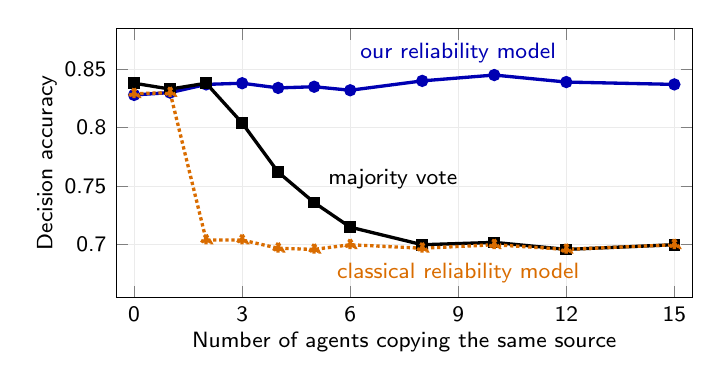
\begin{tikzpicture}
\begin{axis}[width=8.9cm, height=5.0cm, xmin=-0.5, xmax=15.5, ymin=0.655, ymax=0.885,
  xlabel={Number of agents copying the same source}, ylabel={Decision accuracy},
  xlabel style={font=\footnotesize, yshift=3pt}, ylabel style={font=\footnotesize, yshift=-4pt},
  tick label style={font=\footnotesize}, /pgf/number format/assume math mode=true, xtick={0,3,6,9,12,15}, ytick={0.7,0.75,0.8,0.85},
  grid=major, grid style={black!8}, every axis plot/.append style={line width=1.2pt}]
\addplot[blue!70!black, mark=*, mark size=1.6pt] coordinates {(0,0.828) (1,0.830) (2,0.837) (3,0.838) (4,0.834) (5,0.835) (6,0.832) (8,0.840) (10,0.845) (12,0.839) (15,0.837)};
\addplot[black, mark=square*, mark size=1.5pt] coordinates {(0,0.838) (1,0.833) (2,0.838) (3,0.804) (4,0.762) (5,0.736) (6,0.715) (8,0.700) (10,0.702) (12,0.696) (15,0.700)};
\addplot[orange!85!black, densely dotted, mark=triangle*, mark size=1.9pt] coordinates {(0,0.829) (1,0.830) (2,0.704) (3,0.704) (4,0.697) (5,0.696) (6,0.700) (8,0.697) (10,0.700) (12,0.696) (15,0.700)};
\node[font=\footnotesize, anchor=south, inner sep=1pt, text=blue!70!black] at (axis cs:9,0.853) {our reliability model};
\node[font=\footnotesize, anchor=west, inner sep=1pt] at (axis cs:5.3,0.756) {majority vote};
\node[font=\footnotesize, anchor=north, inner sep=1pt, text=orange!85!black] at (axis cs:9,0.687) {classical reliability model};
\end{axis}
\end{tikzpicture}
\end{minipage}\hfill
\begin{minipage}[c]{0.425\textwidth}
\caption{Task~1.1 simulation, averaged over 20 runs of 100 questions. Five independent agents are each right 70\% of the time, and each added agent copies the same source, which is wrong 30\% of the time. Because our reliability model counts the copies about once, the source does not decide the outcome.}
\label{fig:sim}
\end{minipage}
\end{figure}
\hd{Background and challenges.} Before any debate, the protocol must decide which questions deserve one and which agents debate and judge. We identify three challenges. \textbf{First, shared mistakes make a vote overconfident.} Five agreeing agents are five pieces of evidence only if each agent's mistakes are its own. Agents that copy one source are wrong together, so a vote counts their one mistake several times, and such correlated votes can void Condorcet's jury theorem, that adding independent voters makes a majority more often right \citep{ladha1992condorcet}. LLM errors are correlated in practice \citep{kim2025correlated,goel2025great,kohli2026nine}. In Figure~\ref{fig:sim}, agents copying one source drag the majority vote of five independent agents from 84\% to the source's 70\%, and the classical reliability model, which assumes independent mistakes, falls sooner, reading the copies' agreement as skill. \textbf{Second, debate is too costly to run on every question.} It costs three to five times the computation of a single answer and can overturn correct answers \citep{fan2026imad}; yet a unanimous answer can rest on a shared mistake, so neither agreement nor confidence shows which questions need a debate: in one study, most items that discussion helped were unanimous but wrong \citep{hu2026scouting}, and systems that discuss only when agents are unsure \citep{eo2025down} skip exactly those. \textbf{Third, agents that choose debaters and judges can favor themselves.} If agents rate one another to choose a debater for each answer and a judge, an agent can rate rivals low to be chosen, agents built on similar models favor one another's outputs \citep{panickssery2024self,goel2025great}, and a judge that shares a model with one side may favor that side.

\hd{Overview.} RG1 passes to RG2 the question, the two debated answers, their debaters, and the judge. Its two tasks address these challenges, and each controls the terms of Eq.~(\ref{eq:decomp}) that carry its label:
\begin{itemize}
\item Task~1.1 (Figure~\ref{fig:agree}) addresses the first two challenges: its reliability model counts a group that shares a mistake at most once, and a rule derived from expected loss sends a question to debate only when debating is worth the cost.
\item Task~1.2 (Figure~\ref{fig:t12}) addresses the third by choosing the debaters and the judge impartially, so that no agent can use its ratings of others to get itself, or an agent sharing its model, chosen.
\end{itemize}


\subsubsection{Task 1.1: Weighing answers and choosing what to debate}\label{sec:t11}
\hd{Approach.} How much should each answer count when some agents share mistakes, and which questions need a debate? With independent agents, two answers, and equal prior odds, the error-minimizing vote weights an agent that is right with probability $p_a$ by $\log\frac{p_a}{1-p_a}$ \citep{nitzan1982optimal,shapley1984optimizing}, so a weaker agent's answer counts less instead of being discarded: one right 90\% of the time weighs as much as two right 75\% of the time. Classical reliability models estimate these accuracies without an answer key \citep{dawid1979maximum}, as a teacher can grade an exam without the key. When agents make mistakes independently, accurate agents agree often because they are often right, and an agent that keeps disagreeing with the others is likely weak, so how often each pair of agents agrees reveals each agent's accuracy.

Both methods assume independent mistakes. Agents that copy one source are wrong together and agree even when wrong, so the classical reliability model mistakes their agreement for skill. Recent models of dependence among LLM judges \citep{balasubramanian2026ising,zhao2026care} address this for judges that only rate. We adapt the dependent-classifier hierarchy of \citet{jaffe2016dependent} to agents that answer questions: \textbf{a shared-factor reliability model}, a two-level latent-class model fitted to the agents' answers, in which a group that shares a mistake counts at most once. Agents are partitioned into groups $g$, most with one member (in the example, A1 and A2 form one group). On each question, a group has a hidden shared answer $s$, for A1 and A2 what schedule S says, drawn with probability $\kappa_g(s\mid y_q)$; it is the true answer with probability $1-\lambda_g$, so $\lambda_g$ is the chance of a shared mistake. Each member $a$ reports $s$ with its own errors, given by its confusion matrix $\theta_a$, where $\theta_a(x\mid s)$ is the chance that it answers $x$ when the shared answer is $s$. The answers $\mathbf{x}_q$ to question $q$ then have probability
\begin{equation}
P(\mathbf{x}_q\mid y_q)=\prod_{g}\phi_g(y_q),\qquad \phi_g(y)=\sum_{s\in\mathcal{Y}}\kappa_g(s\mid y)\prod_{a\in g\cap A_q}\theta_a(x_{a,q}\mid s),
\label{eq:sharedfactor}
\end{equation}
where $A_q$ is the set of agents that answered $q$, and $\phi_g(y)$ is the probability of the answers of $g$'s members if the true answer is $y$. Decisions use Bayes' rule: the posterior gives each answer's probability given all agents' answers. Two properties of the model explain why it should work. First, a group counts at most once: ten agents reading schedule S can at most establish what S says, and S itself is wrong with probability $\lambda_g$.

% Wrapped figure: it stays at the start of the paragraph below (see README).
\begin{wrapfigure}{r}{0.42\textwidth}
\centering
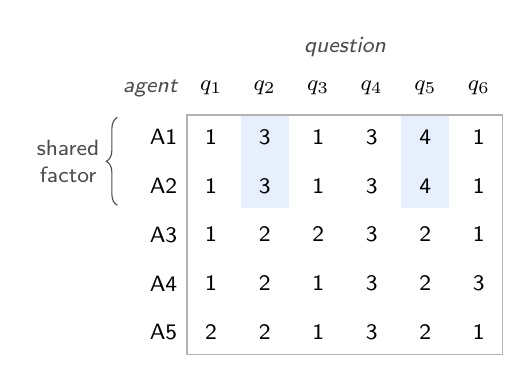
\begin{tikzpicture}[x=0.68cm, y=-0.62cm, font=\footnotesize]
\foreach \q in {1,...,6} \node at (\q,0) {$q_{\q}$};
\foreach \r/\lab in {1/A1,2/A2,3/A3,4/A4,5/A5} \node[anchor=east] at (0.55,\r) {\lab};
% answers: rows are agents A1..A5, columns questions q1..q6 (true answers: 1 2 1 3 2 1)
\foreach \q in {2,5} {\fill[rgfill] (\q-0.45,0.55) rectangle (\q+0.45,2.45);}
\node[anchor=east, font=\footnotesize\itshape, text=black!70] at (0.55,0) {agent};
\node[font=\footnotesize\itshape, text=black!70] at (3.5,-0.85) {question};
\foreach \r/\row in {1/{1,3,1,3,4,1},2/{1,3,1,3,4,1},3/{1,2,2,3,2,1},4/{1,2,1,3,2,3},5/{2,2,1,3,2,1}} {
  \foreach \v [count=\q] in \row { \node at (\q,\r) {\v}; } }
\draw[black!30] (0.55,0.55) rectangle (6.45,5.45);
\draw[decorate, decoration={brace, amplitude=4pt, mirror}, black!70] (-0.75,0.6) -- (-0.75,2.4) node[midway, left=3pt, align=center] {shared\\factor};
\end{tikzpicture}
\caption{Task~1.1 on the running example: agents A1--A5 (rows) answer past questions $q_1$--$q_6$ (columns), and each entry is the number of the answer given. Agents A1 and A2 share unusual answers that no one else gives (shaded), so the reliability model infers a shared factor and counts their agreement about once, without the true answers.}
\label{fig:agree}
\end{wrapfigure}
\textbf{Proposition~1} \textit{(a group counts at most once).} For yes-or-no questions, a group with $0<\lambda_g\le\frac12$ changes the log-odds of the answer by at most $\log\frac{1-\lambda_g}{\lambda_g}$, whatever its size and whatever its members answer. \textit{Proof.} Let $\Lambda$ be the ratio of the probabilities of the members' answers when $s$ is yes and when it is no. By Eq.~(\ref{eq:sharedfactor}), the group's likelihood ratio $\phi_g(\text{yes})/\phi_g(\text{no})$ is $\big[(1-\lambda_g)\Lambda+\lambda_g\big]/\big[(1-\lambda_g)+\lambda_g \Lambda\big]$, which is nondecreasing in $\Lambda$ and lies between $\frac{\lambda_g}{1-\lambda_g}$ and $\frac{1-\lambda_g}{\lambda_g}$.\hfill$\square$

So, under our reliability model, a group carries at most the weight of one agent that is wrong with probability $\lambda_g$, whereas under independence each member would multiply the ratio again. Whether real agents' dependence takes this form is what our experiments test. With more than two answers, wrong ones equally likely, the bound becomes $\log\big[(|\mathcal{Y}|-1)\frac{1-\lambda_g}{\lambda_g}\big]$.

Second, the model can be learned without an answer key. In the simplest case, single agents answering yes or no, with both answers equally likely and symmetric errors, two agents' accuracies $p_a$ and $p_b$ enter their answers only through how often they agree, $p_ap_b+(1-p_a)(1-p_b)$: one number for two unknowns. A third agent adds two more agreement rates, and the three rates determine all three accuracies, up to swapping yes and no.

\textbf{Proposition~2} \textit{(learning without an answer key).} Fix the partition, and suppose every answer has positive prior probability, each group answers a positive share of questions jointly with two other groups, their answers are independent given the true answer, and each group's answer distributions under different true answers are linearly independent (as when its members' confusion matrices are invertible and $\lambda_g<\frac12$). Then each group's distribution of answers given the true answer, which is all the posterior uses, is identifiable, that is, uniquely determined, from the answers alone, up to relabeling. With only two such groups it generally is not: different accuracies fit the answers equally well, so answers alone cannot tell an accurate majority from one that copies a mistake. \textit{Proof sketch.} Given the true answer, three groups answer independently, so the joint distribution of their answers is a three-way array whose factors are the groups' answer distributions; Kruskal's theorem makes such a factorization unique up to relabeling \citep{kruskal1977three,allman2009identifiability}.\hfill$\square$

Answers alone cannot rule out that most agents are wrong with the labels swapped, so we fix the labels and calibrate the posterior on held-out questions with known answers, excluded from fitting; our experiments include pools where the conditions fail. We fit the reliability model over all real questions by expectation--maximization (EM), the standard algorithm for models with hidden variables. Candidate partitions come from clustering agents by agreement on unusual answers: accurate agents agree mostly when they are right, while agents that share a source also give the same wrong answers, as students who copy do \citep{dong2009dependence}. The partition that fits the answers best, with a penalty for extra groups, is kept, and shared sources serve only as clues, since agents can read the same report and reason differently. Topic-specific confusion matrices and question difficulty \citep{whitehill2009whose} keep hard questions from being read as copying. 

\slab{What remains open.} Both propositions take the partition as given. This task's research asks how many questions it takes to detect a group, as a function of its size, $\lambda_g$, and how rarely others give its wrong answers; when the partition itself is identifiable; and how calibration degrades when some agents strategically break the reliability model's assumptions.

\slab{Deciding what to debate.} Recall that $\pi_q$ is the reliability model's probability, from all agents' answers, that the leading answer is right. If the posterior is calibrated (answers given probability $\pi$ are right a fraction $\pi$ of the time), letting the leading answer stand risks the loss $L$ of a wrong decision with probability $1-\pi_q$, an expected loss of $L(1-\pi_q)$. A debate costs $c$ (computation and delay) and, for two answers, ends wrong with probability $\epsilon_D$, at most the bracket in Eq.~(\ref{eq:decomp}), an expected loss of $c+L\epsilon_D$. A debate is worth its cost exactly when $L(1-\pi_q)>c+L\epsilon_D$, that is, when
\begin{equation}
\pi_q<\tau=1-\epsilon_D-c/L.
\label{eq:threshold}
\end{equation}
As $L$ grows, $c/L$ reduces and $\tau$ rises, so the more a wrong answer costs, the more questions go to debate. This is Chow's rule for when to defer a decision \citep{chow1970optimum}, here to a debate. The debate is between the two answers with the highest posterior, so $\epsilon_{\text{cand}}$ is the chance that the right answer is neither; $\epsilon_D$ and $\tau$ are estimated in turn on held-out questions with known answers and posteriors near $\tau$, separately for disputes a tool can settle. Because $\pi_q$ counts each group about once, \textbf{a confident, unanimous answer from agents that share a mistake can still fall below $\tau$ and go to debate}, which rules triggered by the agents' own confidence or by disagreement cannot do.

\hd{Preliminary results.} The simulation in Figure~\ref{fig:sim} supports Propositions~1 and~2. Fitted without the true answers, our reliability model identified the copying agents as one group in 54 of 60 runs (with 2, 6, or 12 copies) and stayed calibrated (calibration error below 0.03). The classical reliability model was overconfident: with two or more copies, it was at least 95\% sure of over 90\% of its decisions, yet 28--30\% of these were wrong. A pilot repeated this with real agents. Nine agents built on four families of publicly released (open-weight) models solved 300 GSM8K problems, and up to four of them received the same hint in their prompts, a suggested answer that was wrong on a third of the problems, like schedule S. With four such agents, majority vote's accuracy on these problems fell from 89\% to 70\% and the classical reliability model's to 71\%, while ours still reached 87\% and identified the four as one group in 9 of 10 runs, so the hint did not decide the outcome.

\hd{Evaluation and risks.} On the math-and-code benchmark (A; Table~\ref{tab:benchmarks}) we inject shared mistakes as in the pilot, and on the multi-document benchmark (B) the source trees fix which reports copy which, so the groups are known. We measure how often the reliability model finds them and after how many questions, and the accuracy and calibration of its decisions, comparing with the classical reliability model, which is ours without shared factors. Our hypothesis, H1, is that our model's advantage over majority vote grows as more agents share a mistake and disappears once fewer than three groups make independent mistakes (Proposition~2); its success criterion, tested by month 24, is a gain of at least 5 points when a third of the agents share a source. The main risk is that EM, our fitting algorithm, settles on a poor solution. We would then start it from a spectral estimate with provable guarantees \citep{zhang2016spectral} or find groups by how alike agents' mistakes are \citep{goel2025great}.

\subsubsection{Task 1.2: Choosing the debaters and the judge impartially}\label{sec:t12}
\hd{Approach.} How can debaters and a judge be chosen so that no agent's ratings of others can get it chosen, at a small cost in quality? Each debate is between two answers, the two with the highest posterior in Task~1.1, so it needs a judge and one debater for each answer, the answer's \emph{representative}. We choose representatives by weighted peer ratings of the arguments behind the agents' answers, as in our PRD and PeerEval \citep{li2024prd}, and make the choice impartial with the partition mechanism of \citet{alon2011sum}, applied to groups: the groups are split at random into two halves, and each answer's representative comes from one half and is rated only by the other. The groups are Task~1.1's, merged when their agents share an underlying model, and are fixed before any rating; $g(a)$ is $a$'s group and $H_q$ the agents that did not answer $q$. Each question takes three steps:
\begin{enumerate}[label=(\arabic*),leftmargin=1.9em]
\item \slab{Draw the judge.} The judge $J$ is drawn uniformly from the $n_q$ agents in $H_q$ with a reliable record on planted debates (debates on questions whose answers we know, Task~2.2); $H_q$ always includes the judges trained in Task~2.1, which never answer. $J$'s group neither debates nor rates.
\item \slab{Split the other groups into two halves.} Each group other than the judge's joins half~1 or half~2 by a fair coin, without regard to ratings, and all its agents go to the same half, so agents that share a model never rate one another. The halves are random sets of groups, not answers, so each half usually holds agents that gave either answer. The coins are redrawn until both halves are nonempty and each debated answer given by two or more of these groups was given by an agent in each half, so that the answer has both candidates and raters.
\item \slab{Choose a representative for each answer.} The leading answer's representative comes from half~1 and the other debated answer's from half~2. For a debated answer $y$, the \emph{candidates} $C_y$ are the agents in $y$'s half that gave $y$, the \emph{raters} $V_y$ are the agents in the other half that gave $y$, and the representative is the candidate with the highest weighted rating:
\begin{equation}
R_y=\mathop{\arg\max}_{a\in C_y}\ \sum_{b\in V_y} w_b\,r_b(a),
\label{eq:rep}
\end{equation}
where $r_b(a)$ is $b$'s rating of $a$'s argument and $w_b$ is $b$'s accuracy as estimated in Task~1.1, not a weight for agreeing with the other raters, which fails once accurate raters are a minority \citep{lev2023peernomination}; ties are broken at random. Agents that gave neither debated answer are neither candidates nor raters. If $C_y$ is empty, as for the other answer when a unanimous answer goes to debate, a random agent of $y$'s half, one that did not answer if possible, argues $y$, as in standard debate; this fallback uses no ratings. Since both halves are nonempty, every debated answer gets a representative, and the two representatives come from different groups.
\end{enumerate}
In the running example (Figure~\ref{fig:t12}), A6, which did not answer, is drawn as judge. The coins put groups G2 (A3) and G4 (A5) in half~1 and G1 (A1, A2) and G3 (A4) in half~2. Yes leads narrowly, so its representative comes from half~1, where A3 is the only agent that gave yes, rated by A1 and A2 in half~2; no's comes from half~2, where A4 gave no, rated by A5. Had the coins swapped G1 and G2, A1 or A2 would argue yes, chosen by A3's ratings. Ratings choose only the debaters; the judge decides the answer.

% Wrapped figure: it stays at the start of the paragraph below (see README).
\begin{wrapfigure}{r}{0.52\textwidth}
\centering
\begin{tikzpicture}[font=\footnotesize,
  grp/.style={draw=taskline, rounded corners=3pt, fill=white, inner sep=2.5pt, align=center, minimum width=2.75cm, minimum height=0.66cm},
  pick/.style={grp, draw=rgline, fill=rgfill, line width=0.9pt},
  ptitle/.style={font=\footnotesize\bfseries, text=rgonedark, anchor=center, inner sep=1pt},
  rate/.style={-{Stealth[length=4.5pt]}, line width=0.8pt, black!65, dashed},
  ratelab/.style={font=\footnotesize\itshape, text=black!60, inner sep=2pt}]
% One panel per debated answer: raters on top, candidates below.
\node[grp] (g1) at (0,0) {half 2, G1: A1, A2\\[-1pt]{\itshape\color{black!65}raters}};
\node[pick] (g2) at (0,-1.5) {half 1, G2: \textbf{A3}\\[-1pt]{\itshape\color{black!65}candidate}};
\node[grp] (g4) at (3.6,0) {half 1, G4: A5\\[-1pt]{\itshape\color{black!65}rater}};
\node[pick] (g3) at (3.6,-1.5) {half 2, G3: \textbf{A4}\\[-1pt]{\itshape\color{black!65}candidate}};
\draw[rate] (g1.south) -- node[ratelab, right]{rate} (g2.north);
\draw[rate] (g4.south) -- node[ratelab, right]{rates} (g3.north);
\begin{scope}[on background layer]
\coordinate (gy) at ([yshift=0.62cm]g1.north); \coordinate (gn) at ([yshift=0.62cm]g4.north);
\node[inner xsep=0.14cm, inner ysep=0.12cm, fit=(g1)(g2)(gy)] (cy) {};
\node[inner xsep=0.14cm, inner ysep=0.12cm, fit=(g4)(g3)(gn)] (cn) {};
\bandpanel{cy}{rgonebg}{rgfill}{rgline}{0.58cm}
\bandpanel{cn}{rgonebg}{rgfill}{rgline}{0.58cm}
\end{scope}
\node[ptitle] at ([yshift=-0.29cm]cy.north) {gave Yes};
\node[ptitle] at ([yshift=-0.29cm]cn.north) {gave No};
\node[pick, minimum width=3.6cm, anchor=north] (j) at ([yshift=-0.3cm]$(cy.south)!0.5!(cn.south)$) {\ico{gavel}\ judge, drawn first, G5: \textbf{A6}};
\end{tikzpicture}
\caption{Task~1.2 on the running example. Agents sharing a model or a source form one group (G1--G5); the judge agent A6 is drawn first. A coin per group splits the other groups into halves, and each answer's debater (bold) is chosen from its agents in one half by its agents in the other, as in Eq.~(\ref{eq:rep}): half~1 supplies Yes's debater, half~2 No's.}
\label{fig:t12}
\end{wrapfigure}
\textbf{Proposition~3} \textit{(impartiality and its price).} (a)~For any group $g$ and any two sets of ratings that differ only in ratings given by members of $g$, each member of $g$ has the same probability of being the judge or a representative. (b)~If each rater's ratings rank agents by argument quality $Q\ge0$ and every weight $w_b$ is positive, then $\mathbb{E}[Q(R_y)]\ge\frac12\,Q(a^*_y)$ for each debated answer $y$ given by two or more groups other than $g(J)$, where $a^*_y$ is the best agent outside $g(J)$ that gave $y$. (c)~If $f$ of the $n_q$ eligible judges collude, a colluder judges with probability $f/n_q$, the least that any lottery can guarantee against every set of $f$ colluders. \textit{Proof.} (a)~$J$, the halves, the fallback draw, and the weights do not depend on current ratings, and Eq.~(\ref{eq:rep}) can choose a member of $g$ only for the answer whose representative comes from $g$'s half, using ratings from the other half alone. (b)~Swapping the two halves preserves the coins' distribution and the redraw condition, so $g(a^*_y)$ lands in $y$'s half with probability exactly $\frac12$; then $a^*_y\in C_y$, $V_y$ is nonempty, and Eq.~(\ref{eq:rep}) selects an agent as good as $a^*_y$. (c)~Under any lottery, the $f$ likeliest agents have total probability at least $f/n_q$.\hfill$\square$

\slab{Why this method.} Part~(a) is impartiality in the usual sense \citep{holzman2013impartial,kurokawa2015impartial}, extended from single agents to groups: no agent's ratings can change the chance that it, or any agent sharing its model, is chosen, so neither self-promotion nor a model's tendency to favor its own outputs \citep{panickssery2024self} can pick the debaters. \textbf{An agent's ratings never count toward its own selection.} Part~(b) makes its price explicit and small: half the best arguer's quality however many groups give the answer, where drawing one of the $K_y$ groups that give $y$ at random guarantees only $1/K_y$. Part~(c) is why judges are drawn uniformly, as in maximally fair panel selection \citep{flanigan2021fair}. \slab{What remains open.} Dishonest agents in different groups can still coordinate their ratings, forming a \emph{coalition}: for example, an agent in half~2 rates its partner in half~1 highest, so that the partner is chosen. Task~2.2's audits look for such collusion; here we will bound what coalitions gain and measure the price of impartiality.

\hd{Preliminary results.} With GPT-4 as the only reviewer, GPT-4's Elo rating (a chess-style rating) was 46 points above the one derived from human preferences, while our weighted peer ranking placed all five models in the human order \citep{li2024prd}. On PeerEval's ratings, a model that rated every rival lowest raised its chance of being chosen as a representative from 0.31 to 0.52 under plain weighted peer ranking and not at all under our mechanism, as Proposition~3(a) guarantees; the mechanism's representatives reached 0.92 of the best arguer's quality, against the 0.5 of Proposition~3(b).

\hd{Evaluation.} On PeerEval and the peer-review benchmark (C), we measure three things: how much the red team's dishonest agents raise their chance of being chosen by misreporting their ratings, alone or in coalitions; the price of impartiality, that is, how much argument quality the chosen representatives give up compared with the best arguer (Proposition~3(b) guarantees at least half in expectation); and the accuracy of the resulting debates. A single dishonest agent gains nothing, by Proposition~3(a). Our hypothesis, H2, tested by month 24, is that coalitions gain less than our bounds allow and that impartiality costs less accuracy than debating adds; its success criterion is that no coalition of two raises its partner's chance of being chosen by more than 0.05, and that the chosen debaters keep at least 0.8 of the best arguer's quality.

\subsection[RG2: Settle Disputes by Agentic Debate, and Audit for Collusion]{\rgsecicon{rg2-comments}RG2: Settle Disputes by Agentic Debate, and Audit for Collusion}\label{sec:rg2}
\suppressfloats[t]% keep the harness figure after the RG2 heading
\begin{figure}[t]
\centering
\begin{tikzpicture}[font=\footnotesize,
  hpart/.style={draw=taskline, rounded corners=3pt, fill=white, align=left, inner sep=3pt, text width=4.2cm},
  lstep/.style={draw=rgtwoline, rounded corners=3pt, fill=auditfill, align=left, inner sep=2pt, text width=4.9cm},
  arr/.style={-{Stealth[length=6pt,width=5pt]}, line width=1.1pt, black!78},
  bigarr/.style={-{Stealth[length=6pt,width=5pt]}, line width=1.3pt, black!85}]
% control loop column
\node[font=\footnotesize\bfseries\itshape, text=rgtwodark] (cl) at (0,0) {\fcico{arrow-sync-24}\ Control loop};
\node[lstep, below=0.12cm of cl] (c1) {1. Each side lays out its argument in numbered steps.};
\node[lstep, below=0.42cm of c1] (c2) {2. Each side names the first step of the other's argument that it disputes.};
\node[lstep, below=0.42cm of c2] (c3) {3. A short exchange on the disputed steps, with tool evidence where a tool applies.};
\node[lstep, below=0.42cm of c3] (c4) {4. Stop. The judge re-runs the evidence and rules on the disputed steps.};
\draw[arr] (c1) -- (c2); \draw[arr] (c2) -- (c3); \draw[arr] (c3) -- (c4);
% left column
\node[hpart, anchor=north east] (ri) at ([xshift=-0.45cm]c1.north west) {\fchead{clipboard-task-24}{Role instructions}Debaters defend one answer, step by step, attaching evidence where a tool applies. The judge rules only on the disputed steps.};
\node[hpart, anchor=north east] (mem) at ([xshift=0cm, yshift=-0.25cm]ri.south east) {\fchead{database-24}{Memory}Logs every message, tool call, and result, for audits and training.};
% right column
\node[hpart, anchor=north west] (sb) at ([xshift=0.45cm]c1.north east) {\fchead{wrench-screwdriver-24}{Sandbox with tools}Document search, structured databases, code execution.};
\node[hpart, anchor=south west] (vf) at (sb.south west |- c4.south) {\fchead{shield-checkmark-24}{Verification}Tool evidence carries its exact call; the judge re-runs it, and evidence that does not reproduce is discarded.};
\begin{scope}[on background layer]
\coordinate (htop) at ([yshift=0.62cm]cl.north);
\node[inner sep=5pt, fit=(cl) (c4) (ri) (mem) (sb) (vf) (htop)] (h) {};
\bandpanel{h}{rgtwobg}{auditfill}{rgtwoline}{0.6cm}
\end{scope}
\node[font=\small\bfseries, text=rgtwodark, inner sep=1pt] at ([yshift=-0.3cm]h.north) {\ico{rg2-comments}\ Agentic debate harness};
\node[anchor=south, font=\footnotesize, inner sep=1pt] (in) at ([yshift=0.55cm]h.north) {\textbf{From RG1:} the question and two answers, \fcico{bot-24}\fcico{bot-24} two debaters, and \fcico{bot-sparkle-24} a judge};
\draw[bigarr] (in.south) -- (h.north);
\draw[arr] (c4.east -| vf.west) -- (c4.east);
\draw[arr] (sb.south west) -- (c3.north east);
\draw[arr] (c3.west) -- (c3.west -| mem.east);
\node[anchor=north, align=center, font=\footnotesize] (out) at ([yshift=-0.28cm]h.south) {\fcico{checkbox-24}\ \textbf{Decision with reasons} $\rightarrow$ audits (Task 2.2) and training (Task 3)};
\draw[bigarr] (c4.south) -- (out.north);
\end{tikzpicture}
\caption{Task~2.1: the agentic debate harness. The control loop sets the order of turns and when to stop, and the judge chosen in Task~1.2 rules on the disputed steps after re-running any tool evidence.}
\label{fig:t21}
\end{figure}
\hd{Background and challenges.} From RG1, RG2 receives a disputed question with its two leading answers, a debater for each, and a judge; it must settle the dispute on evidence, even if some of them collude. Prior peer evaluation by LLMs, in discussion (including our PRD \citep{li2024prd}) and in debate, is an exchange of text: agents speak for a set number of rounds, and a vote or a judge weighs what they wrote \citep{du2024debate,khan2024debating}. Settling disputes on evidence needs more than text: an agentic harness in which agents use tools and a control loop runs the debate. This raises three challenges. \textbf{First, the debaters must back their steps with evidence, and the judge must verify it.} In an exchange of text, a debater can win a step that one database query would settle, or win it with a fake or misreported tool result (Gap~3). In prior peer evaluation by LLMs, agents do not call tools, and no judge re-runs their calls. \textbf{Second, the debate must stop at the steps in dispute.} Open discussion revises until agents agree, and one round can make a panel nearly unanimous without making it more accurate \citep{shu2026unanimity}. In debate theory the judge rules only on a disputed step \citep{irving2018debate,browncohen2024doubly}, but LLM debates follow a fixed schedule of free-form rounds and leave the judge to weigh the whole transcript \citep{khan2024debating,arnesen2024selfplay}, so nothing steers the debate to the steps in dispute. \textbf{Third, debaters or the judge can collude}, by arguing badly on purpose \citep{vanderweij2025sandbagging}, by misleading with true but selectively chosen facts \citep{hu2026lying}, or by favoring one side; re-running evidence catches none of these.

\hd{Overview.} Two tasks address these challenges; each controls the terms of Eq.~(\ref{eq:decomp}) labeled with it:
\begin{itemize}
\item Task~2.1 (Figure~\ref{fig:t21}) addresses the first two with an agentic debate harness, to our knowledge the first for peer evaluation. It is new in two ways: its agents use tools, with debaters gathering evidence through tool calls that the judge re-runs, and its control loop stops the debate at the first step of each argument that the other side disputes, for the judge to rule on. It reduces $\epsilon_{\text{step}}$, the chance that an honest debate still picks the wrong answer.
\item Task~2.2 (Figure~\ref{fig:t22}) addresses the third with automatic audits on planted debates and human audits of random real decisions. With Task~1.2, it reduces $\epsilon_{\text{role}}$, the chance that a dishonest debater or judge steers the outcome.
\end{itemize}


\subsubsection{Task 2.1: Settling disputes by debate before a judge that re-runs evidence}\label{sec:t21}
\hd{Approach.} How can a ruling depend on evidence rather than on persuasion? Debate lets a judge settle a whole question by ruling on single steps: if a side loses whenever one of its disputed steps is ruled false, a judge who rules each disputed step correctly picks the right side \citep{irving2018debate,browncohen2024doubly}.

\textbf{Proposition~4} \textit{(judging a question reduces to judging single steps).} Suppose that (i)~every argument whose steps are all true reaches the right answer, (ii)~the side defending the right answer argues with true steps and can find a false step in the other side's argument, and (iii)~the judge rules correctly on each disputed step. Then, if a side loses exactly when one of its disputed steps is ruled false, the side defending the right answer wins. \textit{Proof.} The other side's argument reaches a wrong answer, so by (i) it contains a false step, which the right side disputes and the judge rules false; any step of the right side's argument that the other side disputes is true, and the judge rules it true.\hfill$\square$

Proposition~4 is why our judge rules only on the disputed steps, never on whole arguments, and it names the three ways a debate can still end wrong, which the harness below is built to prevent. Single steps are what LLMs judge well: checking a reasoning chain one step at a time, each step with only its own premises, raised ChatGPT's verification accuracy to 69\%, from 52\% (about chance) for whole chains \citep{ling2023deductive}. Finding the faulty step is the hard part, since LLMs often fail to locate it but correct it once told where it is \citep{tyen2024llms}; in debate, the opposing side does the locating. In general, a debate ends wrong only if (i) or (ii) fails or one of the judge's $k$ rulings is wrong (one per disputed step), so with $\epsilon_J$ the chance of a wrong ruling on a single step, $\epsilon_{\text{step}}\le P(\text{not (i)})+P(\text{not (ii)})+k\epsilon_J$. A debater or judge that steers the outcome on purpose is counted in $\epsilon_{\text{role}}$ instead, which Tasks~1.2 and~2.2 control.

We propose an \textbf{agentic debate harness}, built so that the assumptions of Proposition~4 hold as often as possible. A harness is the software that turns models into agents \citep{ning2026harness,zhang2026harness,yao2023react,yang2024sweagent}; ours has five parts (Figure~\ref{fig:t21}):
\begin{itemize}
\item \slab{Role instructions} set each debater's answer and its numbered-step format, and limit the judge to disputed steps.
\item The \slab{control loop} sets who speaks and who judges (chosen in Task~1.2) and when to stop: the debaters lay out their arguments, each names the first step of the other's argument that it disputes, a short exchange follows, and the judge rules each disputed step true or false, which enforces the losing rule. The first disputed step is enough, since the disputing side accepts every step before it and the steps after it build on it. Because the loop stops there, rather than after a set number of rounds, the disagreement that exposes the error survives until the judge rules.
\item \slab{Tools}, such as document search, databases, and code execution, let the debaters back their steps with evidence; steps that no tool can settle are argued in text.
\item \slab{Verification} supports assumption~(iii) of Proposition~4, that the judge rules correctly on each disputed step: tool evidence carries its exact call (tool, arguments, data version), which the judge, itself an agent \citep{zhuge2025agent}, re-runs, and evidence that does not reproduce is discarded. Re-running proves an output authentic, so if the query fits the claim and the data are current, it settles the step.
\item \slab{Memory} logs every message, call, and result, for audits (Task~2.2) and training (Task~3).
\end{itemize}

The harness also supports assumptions~(i) and~(ii) of Proposition~4. Assumption~(i), that an argument whose steps are all true reaches the right answer, fails when true but selectively chosen facts lead to a wrong answer \citep{hu2026lying}, so each side has a right of reply: it may add context to the other side's evidence before the judge rules, and quotations are verified against the source \citep{khan2024debating}. Assumption~(ii), that the side with the right answer can find a false step in the other side's argument, is the hard part noted above; a disputed step too complex to rule on is broken into sub-steps, and the debate continues on the one in dispute, which narrows the search \citep{browncohen2025prover}. In the vessel example, A4 disputes A3's step ``so V left at 06:00'' with a port report, whose query the judge re-runs (Figure~\ref{fig:overview}).

\slab{Training the judges.} Re-running lowers $\epsilon_J$ only on steps a tool can settle; on the others the judge rules on argument alone, so we further train several open-weight judges to rule on single steps, first on human labels of steps and of debates \citep{lightman2024verify,michael2023debate,khan2024debating}, then by reinforcement learning on debates over questions with known answers, never on the agents' decisions or planted cases.

\hd{Preliminary results.} In 50 pilot debates in our simplified harness, on questions where a calculator or database query could check the disputed steps, the judge ruled correctly in 94\% of them.

\hd{Evaluation and risks.} On the multi-document (B) and peer-review (C) benchmarks, we measure accuracy on disputed questions, how often re-running evidence changes the outcome, and cost. Our hypothesis, H3, tested by month 24, is that debate is more accurate than open discussion among the same agents and, where a tool can settle the disputed steps, than every baseline, more so as the share of such steps grows; its success criterion is that the judge rules correctly in at least 90\% of disputes a tool can settle, and that debate is at least 5 points more accurate than open discussion on them. If a tool can settle few disputed steps, rulings rest on argument and on the judges' training.

\subsubsection{Task 2.2: Auditing for collusion with planted cases and human audits}\label{sec:t22}
\hd{Approach.} How can colluding debaters or judges be caught when people check only a small, fixed share of decisions? Collusion shows up as a debater that fails to expose a clear flaw or a judge that rules against clear evidence, so we check for exactly that, with two simple checks based on random inspection \citep{avenhaus2002inspection} (Figure~\ref{fig:t22}).

% Figure 7: a float with the caption beside the diagram (as a wrapfigure it kept running off the page when text reflowed).
\begin{figure}[t]
\begin{minipage}[c]{0.44\textwidth}
\centering
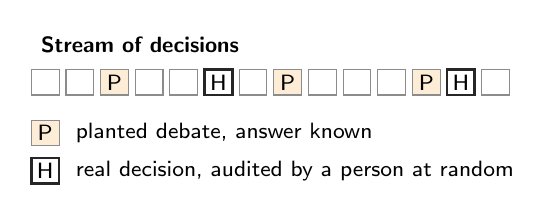
\begin{tikzpicture}[font=\footnotesize, x=0.44cm, y=0.40cm]
\node[anchor=west, font=\footnotesize\bfseries] at (0,1.6) {Stream of decisions};
\foreach \i in {1,...,14} {\draw[black!45, fill=white] (\i-1,0) rectangle (\i-0.2,0.8);}
\foreach \i in {3,8,12} {\draw[black!45, fill=auditfill] (\i-1,0) rectangle (\i-0.2,0.8); \node at (\i-0.6,0.4) {P};}
\foreach \i in {6,13} {\draw[black!85, line width=1pt] (\i-1,0) rectangle (\i-0.2,0.8); \node at (\i-0.6,0.4) {H};}
\draw[black!45, fill=auditfill] (0,-1.6) rectangle (0.8,-0.8); \node at (0.4,-1.2) {P};
\node[anchor=west, font=\footnotesize] at (1.0,-1.2) {planted debate, answer known};
\draw[black!85, line width=1pt] (0,-2.8) rectangle (0.8,-2.0); \node at (0.4,-2.4) {H};
\node[anchor=west, font=\footnotesize] at (1.0,-2.4) {real decision, audited by a person at random};
\end{tikzpicture}
\end{minipage}\hfill
\begin{minipage}[c]{0.53\textwidth}
\caption{Task~2.2: two kinds of audits. Planted debates (P), whose answers are known, are mixed into the stream, and human audits (H) check a few real decisions drawn at random afterward; an agent that fails either check is disqualified.}
\label{fig:t22}
\end{minipage}
\end{figure}
\slab{Planted debates.} We mix into the stream debates on planted cases, whose answers are known and easy to defend because the other answer rests on a planted flaw, such as a changed timestamp in a port report or an error inserted into a paper \citep{schroter2008errors}. The debater for the right answer should expose the flaw, and the judge should rule for that side; an agent that fails on such easy cases is flagged. Planted cases help only if they cannot be told from real questions \citep{checco2018gold}, and capable LLMs often tell evaluations from real use \citep{needham2025evaluated}, so we build them from real questions by controlled edits and keep only those that a classifier trained to spot them cannot tell from real ones.

\slab{Human audits.} A colluder that recognizes planted debates can behave well on them, so a person or a direct measurement, such as a satellite image, also checks a few real decisions drawn at random after they are made; no agent can know which, just as random tax audits deter evasion \citep{allingham1972tax,gans2026randomized}. An agent whose audited real decisions go wrong much more often than its estimated accuracy predicts is flagged, by a test rechecked after every audit that keeps the chance of ever flagging an honest agent below a chosen level $\alpha$ \citep{ramdas2023game}; the number of audits needed does not grow with the number of decisions \citep{steinhardt2016avoiding}. Flagged agents are disqualified: they lose their weight in Task~1.1 and may no longer debate or judge.

\slab{Bounding the harm.} Treating auditing as an inspection game, in which audits are random and the colluder chooses when to cheat, we expect to bound the harm it can do before it is flagged. If honest agents make no mistakes, a colluder's first audited wrong decision exposes it, so its harm is of order $1/\rho$ at audit rate $\rho$, however long the stream. If they do, it can hide among their mistakes, and we expect a bound of order $\sqrt{n\log\log n/\rho}$ wrong decisions beyond the honest error rate in $n$ decisions, the slack any such test must allow \citep{howard2021timeuniform}. We will prove such bounds and compare them with the red team's best attacks. A colluder that mimics a weak honest agent is never flagged, but a weak agent earns little weight (Task~1.1) and no seat as judge (Task~1.2).
\hd{Preliminary results.} In a pilot in our simplified harness, planted debates flagged 90\% of the debaters and judges that we told to collude, and no honest agent.
% Confirm 90% and "no honest agent" against the pilot before submission.

\hd{Evaluation.} Against the red team, we measure the share of colluders flagged and how soon, false flags, wrong decisions that get through at each audit budget, and whether a classifier can tell planted cases from real ones. Our hypothesis, H4, tested by month 36, is that colluders cheating at a fixed rate are flagged after a number of audits that does not grow with the stream, with false flags below the chosen level; its success criterion is that at least 90\% of colluders that do not coordinate across roles are flagged, with false flags below $\alpha=0.05$.

\subsection[RG3: Self-Improve with Reinforcement Learning on Collective Decisions]{\rgsecicon{rg3-graduation-cap}RG3: Self-Improve with Reinforcement Learning on Collective Decisions}\label{sec:rg3}
\hd{Background and challenges.} From RG1 and RG2, RG3 receives each decision with its reasons and trains the agents on these decisions. Reinforcement learning (RL) updates a model so that answers earning high reward become more likely; with verifiable rewards (RLVR), the reward comes from an answer key, as in math and code \citep{lambert2024tulu}. RG3 extends such training to questions without one, such as whether vessel V has left port. It focuses on decisions the judge settled by re-running tool evidence: debate narrows a question to steps a tool can check (RG2), so these decisions are grounded and verifiable, like an executed test for code, and usually correct (94\% in our Task~2.1 pilot). The rewards must come from these collective decisions yet still track correct answers, which raises two challenges. \textbf{First, the obvious label-free rewards can be gamed.} Training a model on its own majority answers \citep{huang2023selfimprove,zuo2025ttrl} rewards conformity and can collapse accuracy \citep{shafayat2025selftrain,he2026urlvr}, rewarding debate wins can teach debaters to exploit the judge \citep{kenton2026debate}, and rewarding approval favors misleading the evaluator \citep{wen2025mislead}. \textbf{Second, the agents' own decisions are imperfect labels.} Training on a wrong decision could reinforce the behavior that produced it, and existing label-free methods assume that models' mistakes differ \citep{yang2026corl}.

\hd{Overview.} Task~3 addresses both with two rewards that need no human labels; by lowering the agents' own error rates, it can reduce every term of Eq.~(\ref{eq:decomp}):
\begin{itemize}
\item The \emph{answer reward} of Eq.~(\ref{eq:firstanswer}) rewards each agent's answer for matching a reference the agent did not shape: the decision, if the judge settled the question by re-running tool evidence, and otherwise the answer the other groups favor. It gives the true answer the highest average reward whenever the reference is right more often than wrong.
\item The \emph{message credit} of Eq.~(\ref{eq:credit}) credits each debate message by how far it moved the judge toward the decision, only in debates the judge settled by re-running tool evidence, so the credit rests on verifiable evidence rather than persuasion.
\end{itemize}

\subsubsection{Task 3: Rewarding each agent's contribution to collective decisions}\label{sec:t3}
\hd{Approach.} What reward makes agents more accurate when the only labels are the agents' own, imperfect decisions? \textbf{We first select which decisions to learn from}: mainly those the judge settled by re-running tool evidence, and, where no tool settled a question, the answer the other groups favor, a noisier label. Because these labels can still be wrong, especially the fallback, we treat each decision as a noisy label \citep{natarajan2013noisy}. Suppose an agent earns a reward of 1 when its answer to a yes-or-no question matches a reference answer, and 0 otherwise, and the reference is wrong with probability $\eta_q$, whatever the agent answers. A right answer then matches the reference with probability $1-\eta_q$, and a wrong answer with probability $\eta_q$ (when the reference is wrong too). So \textbf{a right answer still earns more on average}, by $1-2\eta_q$, whenever $\eta_q<\frac12$ (0.8 against 0.2 when $\eta_q=0.2$), and training on this reward moves the agent the same way as training on the true answer, with an expected update $1-2\eta_q$ times as large. This requires that the reference's mistakes do not depend on the agent's answer: a reference that includes the agent's own answer is wrong more often exactly when the agent is, which is how rewards for majority agreement collapse \citep{shafayat2025selftrain}. We propose two rewards that meet it. Task~3 updates the open-weight models behind the agents: the answer reward trains every agent that answered, and message credit trains the two debaters; the judge only scores the debate and is never trained on collective decisions (Task~2.1).

\slab{Answers.} Agent $a$'s answer $x_{a,q}$ to question $q$ is scored against a reference $\tilde D_{a,q}$ chosen so that its mistakes do not depend on $a$'s answer. If the judge settled $q$ by re-running tool evidence, the reference is the decision $D_q$; the two debaters, whose arguments shaped it, earn only message credit on $q$. Otherwise the reference is the answer that the posterior of Task~1.1 favors when $a$'s group (Task~1.2) is left out, which counts shared mistakes once and discounts flagged agents. References are frozen during each update phase. The reward is
\begin{equation}
\mathrm{reward}_a(q)=\omega_{a,q}\,\mathbf{1}\{x_{a,q}=\tilde D_{a,q}\},
\label{eq:firstanswer}
\end{equation}
where $\mathbf{1}\{\cdot\}$ is 1 if the answer matches the reference and 0 otherwise, and the weight $\omega_{a,q}=1-2\hat\eta_{a,q}$ lets questions with a more reliable reference count more and, unlike dividing by $1-2\hat\eta_{a,q}$ to restore the full update \citep{natarajan2013noisy}, never amplifies a noisy reference. Here $\hat\eta_{a,q}$ estimates the chance that the reference is wrong, from the judge's calibrated probability or the left-out posterior (with more answers, $\omega_{a,q}$ is the gap between the two likeliest answers' probabilities).

\slab{Debate messages.} Each message $m_t$ is credited by how far it moves the judge toward the decision:
\begin{equation}
\mathrm{credit}_t=\omega_q\,\big[\,P_J(D_q\mid m_{1:t})-P_J(D_q\mid m_{1:t-1})\,\big],
\label{eq:credit}
\end{equation}
where $P_J(D_q\mid m_{1:t})$ is the judge's probability of the decision when shown only the first $t$ messages of the debate, and $\omega_q=1-2\hat\eta_q$, with $\hat\eta_q$ the judge's calibrated probability that $D_q$ is wrong. A message that makes the judge more sure of the decision earns positive credit, and one that makes it less sure, negative credit. Each message is thus credited with its effect given the earlier ones \citep{wolpert2001optimal,agogino2008analyzing}.

A persuasive message can move the judge toward a wrong decision, so messages are credited only in debates the judge settled by re-running tool evidence. By the argument above, on yes-or-no questions a message's expected credit is a positive multiple of how far it moved the judge toward the true answer, provided such decisions are right more often than wrong and whether one is right does not depend on that move. A decision settled by argument alone is not used as a label: after such a debate, answers are scored against the other groups' answers, and messages earn no credit.

For both rewards, decisions involving agents already flagged are dropped, planted cases never enter training (R5), and no agent is trained on its own rulings or shares a reward with an agent that judges it \citep{shi2026collusion}. Task~2.2's random human audits estimate each topic's error rate, and training on a topic stops once the audits show that rate above a preset threshold below one half, as both need.

\hd{Preliminary results.} In a pilot training a 1.5B-parameter model on GSM8K, with three of the eight agents whose answers form the reference sharing a flawed hint, rewarding agreement with the model's own majority answers raised held-out accuracy and then collapsed it, while the reward of Eq.~(\ref{eq:firstanswer}) raised it from 55\% to 73\% without collapse.

\hd{Evaluation.} On all three benchmarks, we train the same models with our rewards, with rewards for majority agreement and for debate wins \citep{arnesen2024selfplay}, and, as an upper bound, on the known answers (standard RLVR); otherwise the known answers are used only for evaluation. We compare the accuracy of the agents' answers and of the collective decisions on held-out questions. The known answers also show how often the references are wrong, by topic, testing the premise $\eta_q<\frac12$ directly. Our hypothesis, H5, tested by month 36, is that our rewards gain more than majority-agreement and debate-win rewards and recover at least half the gain of training on the known answers.

\subsection{Shared Evaluation Setup and Expected Results}\label{sec:eval}
Each task states its own evaluation and hypothesis (H1--H5); this section gives what the tasks share.


\hd{Agent pools and red team.} Agents are built on open-weight models of several families and sizes, plus commercial models where licenses allow, with varied role instructions and tools. Our red team, modeled on AI control evaluations \citep{greenblatt2024control}, builds attackers of increasing strength, from a single dishonest agent, through agents that know the protocol or learn to spot planted debates and cheat only when they expect no audit, to a debater and a judge that coordinate through hidden signals. We report the wrong decisions that get through at each audit budget against the useful work still done, as safety--usefulness curves.

\hd{Conditions, baselines, and statistics.} Experiments vary how widely mistakes are shared (from none to most agents given the same flawed hint or outdated report, across one to five model families), the share of dishonest agents (up to 30\%, against each attacker), the share of disputed steps a tool can settle and of reports that are outdated or forged, the budgets for debates, audits, and computation (including small models and few tool calls, as under limited connectivity), and the answer type. Regimes where the propositions say a method fails are included, so that failures are measured; transfer is measured on held-out topics and model families. Baselines at matched compute are a single AI judge (with and without the debaters' tools), majority vote, open discussion, and equal-weight averaging; ablations remove one component at a time, and each term of Eq.~(\ref{eq:decomp}) is measured separately, so a gain can be traced to the task that produced it. Benchmark B also reports the running example's measure, missed and false departure calls per 100 vessel questions at each audit budget. We report accuracy, calibration (Brier score, expected calibration error), and means with confidence intervals over seeds and questions.

\label{sec:expected}\hd{Results and new knowledge.} If successful, the project will deliver the methods of Section~\ref{sec:merit} with their theory (identifiability without an answer key, the price of impartiality, bounds on coalition gains and on a colluder's harm, and rewards that move agents toward correct answers on average), an open debate harness, three benchmarks, and red-team protocols. Scientifically, it will show when a debate among AI agents can be trusted and how few audits keep the agents honest, which would let conferences and funders try impartial, audited peer review by AI; because people audit only a small share of decisions and training needs no labels, the methods can scale to AI whose answers people cannot easily evaluate.

\subsection{Project Schedule, Milestones, Goals, and Benchmarks}\label{sec:schedule}
The project runs 36 months from April 1, 2027, with milestones M1--M6 (Table~\ref{tab:schedule}).
% Schedule table: [H] = exactly here, inside Section 2.6 (not floated to another page).
% Gantt bars: grey for benchmarks and red team, one color per research goal (as in the figures).
\newcommand{\g}{\cellcolor{black!22}}\newcommand{\gA}{\cellcolor{rgline}}\newcommand{\gB}{\cellcolor{rgtwoline}}\newcommand{\gC}{\cellcolor{goodline}}
\begin{table}[H]
\centering\small
\renewcommand{\arraystretch}{1.05}
\setlength{\tabcolsep}{4pt}
\begin{tabularx}{\textwidth}{@{}Xcccccc}
\toprule
Activity & Y1a & Y1b & Y2a & Y2b & Y3a & Y3b\\
\midrule
\multicolumn{7}{@{}l}{\textbf{Benchmarks and red team} (Sections~\ref{sec:setting} and~\ref{sec:eval})}\\
\hspace{0.8em}Benchmarks A and B; simple attackers & \g & \g & & & & \\
\hspace{0.8em}Benchmark C; attackers that spot planted debates & & & \g & \g & & \\
\hspace{0.8em}Coordinating attackers; full evaluation; release & & & & & \g & \g\\
\addlinespace[2pt]
\multicolumn{7}{@{}l}{\textbf{\color{rgonedark}RG1: Weigh answers, and choose the debaters and the judge}}\\
\hspace{0.8em}Task 1.1: reliability model, identifiability; then topics, error costs & \gA & \gA & \gA & & & \\
\hspace{0.8em}Task 1.2: impartial choice; then coalitions, price of impartiality & & \gA & \gA & \gA & & \\
\addlinespace[2pt]
\multicolumn{7}{@{}l}{\textbf{\color{rgtwodark}RG2: Settle disputes by agentic debate, and audit for collusion}}\\
\hspace{0.8em}Task 2.1: harness and judges; then sub-step recursion, right of reply & \gB & \gB & \gB & \gB & & \\
\hspace{0.8em}Task 2.2: planted and human audits; then audit bounds & & & \gB & \gB & \gB & \\
\addlinespace[2pt]
\multicolumn{7}{@{}l}{\textbf{\color{rgthreedark}RG3: Self-improve with reinforcement learning on collective decisions}}\\
\hspace{0.8em}Task 3: rewards (\ref{eq:firstanswer})--(\ref{eq:credit}); then comparison & & & & \gC & \gC & \gC\\
\midrule
\multicolumn{7}{@{}p{\dimexpr\textwidth}@{}}{\textbf{Milestones.} M1 (month 6): harness v1 and benchmark A released. M2 (12): reliability model and its identifiability analysis, on benchmarks A and B. M3 (18): impartial choice of debaters and judges integrated; tool-backed debate on benchmark B. M4 (24): audit scheme against attackers that do not coordinate across roles; benchmark C; H1--H3 tested. M5 (30): audit bounds; analysis and comparison of rewards. M6 (36): full framework against coordinating attackers; H4--H5 tested; code, benchmarks, and protocols released.}\\
\bottomrule
\end{tabularx}
\caption{Schedule by half-year (Y1 = April 2027 to March 2028) and milestones.}
\label{tab:schedule}
\end{table}

\label{sec:goalsbench}\hd{Goals and benchmarks.} The research goals are RG1--RG3 (Section~\ref{sec:goals}). Progress toward them is measured on benchmarks A--C (Table~\ref{tab:benchmarks}) and PeerEval against the success criteria of hypotheses H1--H5, each stated with its target in its task's evaluation (Sections~\ref{sec:rg1}--\ref{sec:rg3}). Targets sit near or below the pilot results because they must hold on harder benchmarks and against stronger red teams than the pilots faced. H1--H3 are tested at M4 (month 24) and H4--H5 at M6 (month 36), with interim results at other milestones and the annual Program Reviews; misses are reported as findings. Code, benchmarks, protocols, and peer-reviewed papers with proofs are released by month 36.




\subsection{Gold Standard Science}\label{sec:gss}
The PI's group already follows the tenets of Executive Order 14303: MEQA, DSBench, and LMR-Bench were released with their data and code \citep{li2024meqa,jing2025dsbench,yan2025lmrbench}, and OpenAI has since used DSBench to evaluate ChatGPT agent \citep{openai2025agent}. This project continues that practice: every debate is logged with exact tool calls, prompts, and seeds for re-running; code, benchmarks, and protocols are released with each paper; guarantees are stated with their assumptions; hypotheses H1--H5 and analysis plans are fixed in advance; a red team attacks our own methods; and negative results are published.

\section{Management Approach}\label{sec:mgmt}
This is a single-PI award with no subawardees, collaborators, co-investigators, or senior personnel. The PI directs all research, submits annual and final reports, attends ONR Program Reviews, and publishes in peer-reviewed venues, releasing code, benchmarks, and protocols at M1, M6, and with each paper. The budget supports two Ph.D.\ students for three years, one month of PI summer effort per year, travel to ONR Project and Program Review Meetings and to conferences, and cloud computing and model access.

Student~1 (statistics and mechanism design) leads Tasks~1.1 and~1.2, the audit analysis of Task~2.2, and benchmarks A and C. Student~2 (LLM agents and reinforcement learning) leads the harness and trained judges of Task~2.1, the planted-case generator of Task~2.2, Task~3, and benchmark B. Both run the red team, rotating roles so that no one attacks only their own method. The PI meets each student weekly and reviews progress against the milestones (Table~\ref{tab:schedule}) and the success criteria of H1--H5 every six months.

\section{Principal Investigator Qualifications}\label{sec:pi}
The PI, Xinya Du, has been an Assistant Professor of Computer Science at The University of Texas at Dallas since 2022, after a Ph.D.\ in Computer Science from Cornell University (2021, advised by Claire Cardie) and postdoctoral research with Heng Ji at the University of Illinois Urbana-Champaign. The PI has 66 papers and preprints, including 28 in the main proceedings of NeurIPS, ICLR, ICML, ACL, EMNLP, NAACL, EACL, and AAAI, cited 4,735 times (h-index 29, Google Scholar, October 2026); \$1.02M in external research funding as sole PI; and three Ph.D.\ students, two finishing in 2026, with former mentees now in Ph.D.\ programs at CMU, Cornell, and NTU. The most pertinent contributions, most of them made with students at UT Dallas, are these:

\hd{Peer evaluation among AI judges.} PRD \citep{li2024prd} introduced peer ranking and peer discussion among AI judges, which agree with human judgments better than the strongest single judge and reduce a judge's bias toward its own model; researchers at NYU, Anthropic, and Cohere have built on it. It underlies PeerEval (\href{https://peereval-ai.github.io}{peereval-ai.github.io}), a public leaderboard on which seven AI models answer the same questions and judge one another anonymously (40,156 pairwise judgments in its first release). IQA-EVAL \citep{li2024iqa} lets AI agents with assigned personas play the users of an interactive question-answering system and then evaluate the interactions, agreeing closely with human evaluators. PRD and PeerEval are the basis for Task~1.2's weighted peer ratings and its preliminary results, and IQA-EVAL supports giving the agents of Section~\ref{sec:eval} varied role instructions.

\hd{Faithfulness evaluation across modalities.} FaithScore \citep{jing2024faithscore} splits a vision-language model's free-form answer into atomic facts and checks each against the image; groups at Arizona State, the University of Washington, Johns Hopkins, and Intel Labs have adopted it. FIFA \citep{jing2026fifa} extends such fact-level checks to text-to-video and video-to-text generation, agreeing with human judgment more closely than earlier methods. FIHA \citep{yan2025fiha} evaluates hallucinations in vision-language models automatically with scene graphs, and Dr.V \citep{luo2026drv} diagnoses video hallucinations by grounding them in space and time. Checking one claim at a time against evidence is also how Task~2.1's judge rules on each disputed step.

\hd{Step-level rewards and verification.} FG-PRM \citep{li2025fgprm} detects six types of hallucination at each step of a math solution, and HiPRAG \citep{wu2026hiprag} rewards each search decision of an agent, cutting needless searches to 2.3\% and missing fewer needed ones. HiPRAG underlies Task~3's message credit.

\hd{Question generation and benchmarks.} A paper from the PI's Ph.D.\ on neural question generation \citep{du2017learning} has been cited more than 1,000 times and is ranked by Paper Digest among the most influential ACL 2017 papers. MEQA \citep{li2024meqa} composes multi-hop questions with explanations from event structures and builds benchmark B. DSBench \citep{jing2025dsbench}, which OpenAI used to evaluate ChatGPT agent \citep{openai2025agent}, and LMR-Bench \citep{yan2025lmrbench} test agents that analyze data and reproduce research code, the kind of tool use that Task~2.1's judge re-runs and benchmark C checks.

\hd{Adversarial evaluation.} The PI co-advised one of the five university red teams in the Amazon Nova AI Challenge \citep{sahai2025nova,comet2025}, whose findings shape Task~2.2's planted cases, and holds an Open Philanthropy grant on control evaluations of AI debate.

The PI's awards include the NSF CAREER Award (2024--2029, funded on first submission), Amazon (2023) and Cisco (2024) Research Awards, the Best Paper Award of the AAAI 2025 AI4Research Workshop, AAAI New Faculty Highlights (2024), and the University of Chicago Rising Star in Data Science (2021). The PI is an area chair for ICML 2027, ICLR 2027, and NeurIPS 2026, has been one for ICLR 2025, ACL, EMNLP (Outstanding Area Chair Award, 2024), and COLING, and has served on NSF review panels, including for CAREER. As a postdoctoral researcher, the PI led the integration of RESIN, the event-prediction system built under a \$10M DARPA KAIROS grant and ranked first in its evaluation, and was first author of RESIN-11 \citep{du2022resin}.

\section{Responsibility}\label{sec:resp}
\hd{Resources.} UT Dallas provides the PI's laboratory space, a GPU server (ten A100 GPUs), and the shared Juno cluster (67 GPUs; see Facilities and Other Resources). With the requested cloud and model-access costs, these suffice; no equipment purchase is requested. \hd{Ability to comply.} The UT Dallas Office of Research and Innovation administers the PI's federal awards and will administer this award under 2 CFR 200 and ONR terms; the PI's commitments, listed in Current and Pending Support, leave the proposed effort available.

\hd{Performance history.} The PI has managed an NSF CAREER award (2024--2029) and industry and foundation awards, filing reports on time; funds on current awards are being spent on schedule.

\hd{Integrity and business ethics.} The PI and UT Dallas follow federal research-integrity policies (DoDI 3210.7); the PI has no record of misconduct. \hd{Qualifications and eligibility.} The PI is a U.S.\ permanent resident, has held a full-time tenure-track appointment at UT Dallas since 2022, the PI's first, and received the Ph.D.\ from Cornell University in 2021, on or after January 1, 2019, as Section B of the NOFO requires. \hd{Organization and controls.} UT Dallas maintains federally reviewed accounting, property-control, research-security, quality-assurance, and safety systems and is registered in SAM (UEI EJCVPNN1WFS5; CAGE 0W921); the research is computational.
\label{techend}

% ---------------- CV and letters of support (not counted) ----------------
\clearpage
\renewcommand{\thepage}{CV-\arabic{page}}
\setcounter{page}{1}
\refstepcounter{section}\phantomsection\addcontentsline{toc}{section}{\protect\numberline{\thesection}Principal Investigator's Curriculum Vitae}
% \includepdf drops the CV's own links; cv_links.tex (from cv_links.py) puts them back over each page.
\newcount\cvpage \cvpage=0
\newcommand{\cvlinkspage}{\global\advance\cvpage by 1 \setlength{\unitlength}{1bp}\csname cvlinks@p\the\cvpage\endcsname}
\InputIfFileExists{cv_links.tex}{}{}
\IfFileExists{cv_onr.pdf}{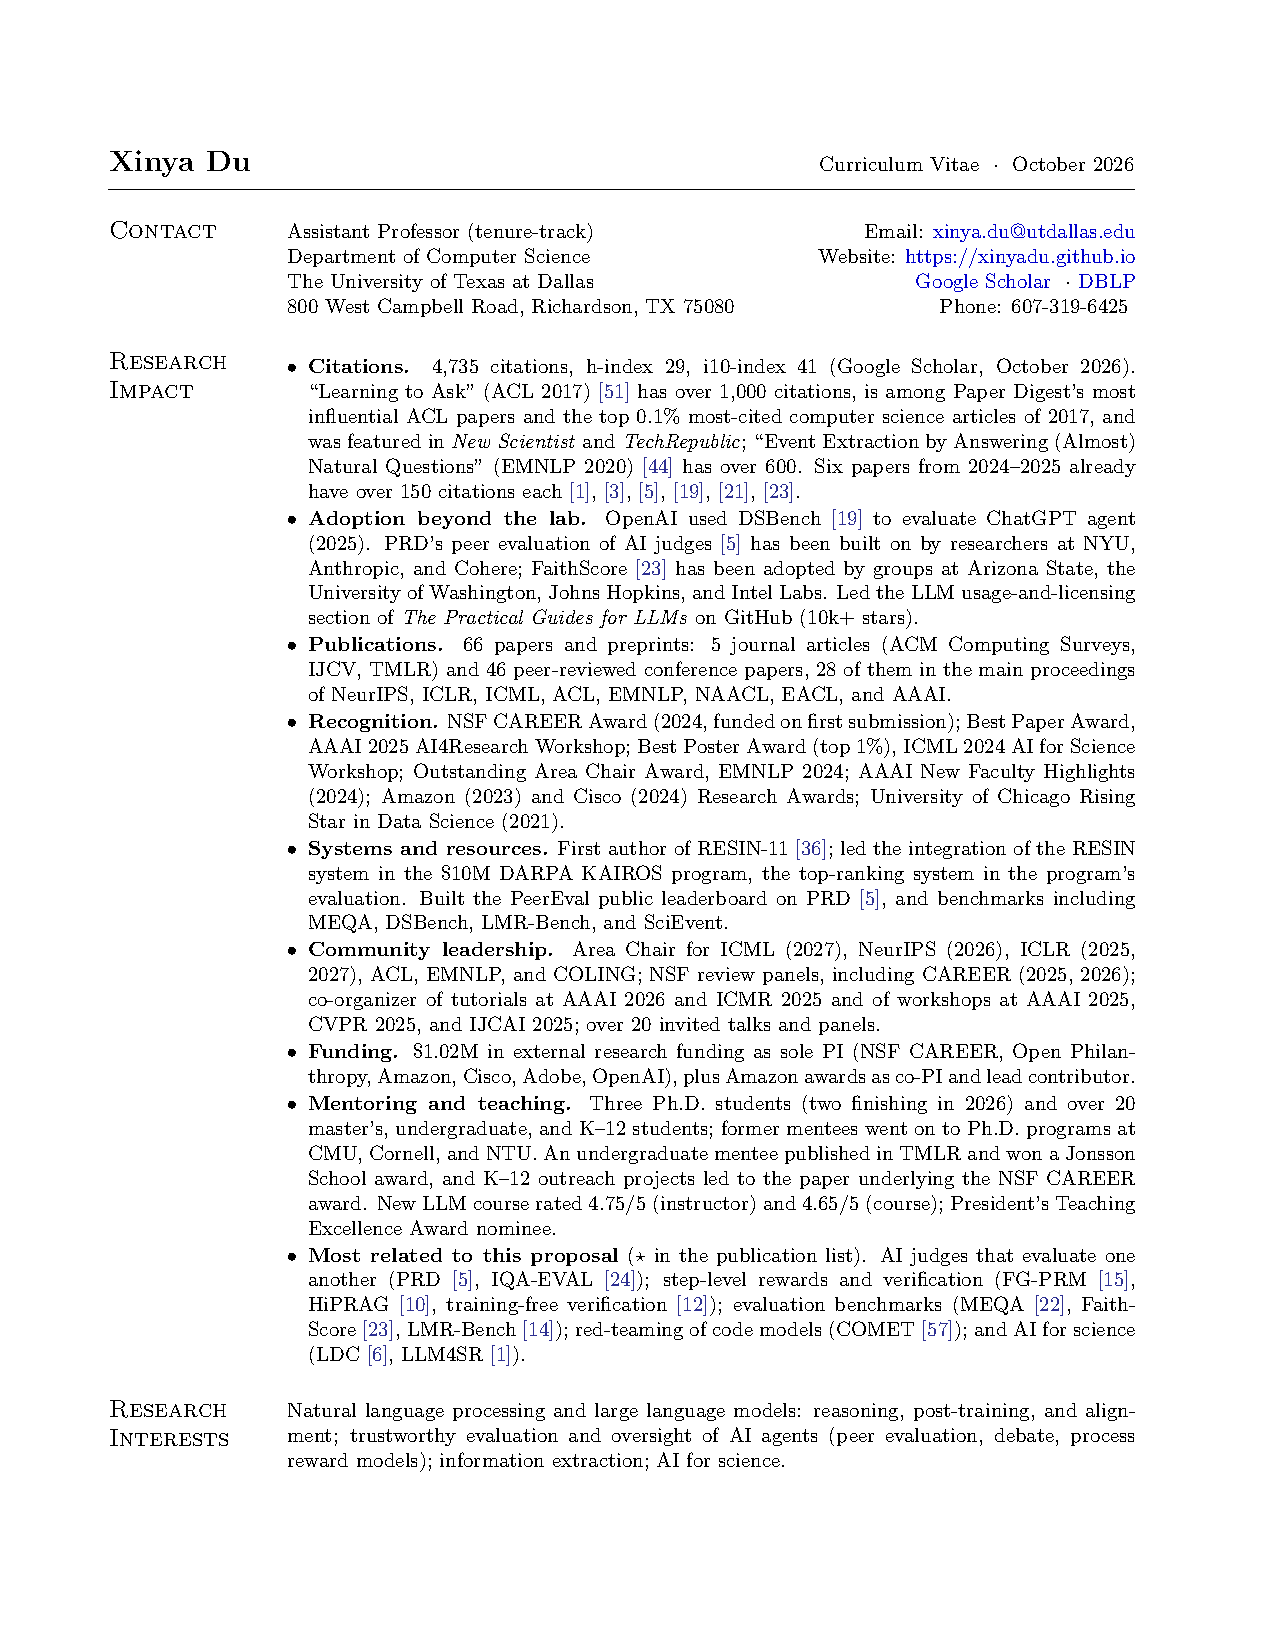
\includepdf[pages=-,pagecommand={\thispagestyle{plain}},picturecommand={\cvlinkspage}]{cv_onr.pdf}}{\section*{Principal Investigator's Curriculum Vitae}\confirm{[Add cv\_onr.pdf (the PI's full CV) to this folder; it is inserted here.]}}

\clearpage
\renewcommand{\thepage}{LS-\arabic{page}}
\setcounter{page}{1}
\refstepcounter{section}\phantomsection\addcontentsline{toc}{section}{\protect\numberline{\thesection}Letter(s) of Support}
\IfFileExists{DU-LOR-ONR-YIP-signed.pdf}{
\includepdf[pages=-,pagecommand={\thispagestyle{plain}}]{DU-LOR-ONR-YIP-signed.pdf}}{\section*{Letter(s) of Support}\confirm{[Add DU-LOR-ONR-YIP-signed.pdf (letter from Dr.\ Rym Zalila-Wenkstern, Interim Department Head) to this folder; it is inserted here.]}}

% ---------------- Data management plan (not counted; at most 2 pages) ----------------
\clearpage
\renewcommand{\thepage}{DMP-\arabic{page}}
\setcounter{page}{1}
\section{Data Management Plan}\label{sec:dmp}
\small
\hd{Types of data, software, and other materials.} The project will produce (1)~three benchmarks of questions with known answers: math and code problems with injected shared mistakes (A), multi-document questions composed from event structures, including synthetic maritime scenarios (B), and scientific-claim and peer-review questions with inserted errors (C); (2)~logs of agent answers, ratings, debates, tool calls and their outputs, judge rulings, and audit outcomes; (3)~software: the agentic debate harness, the shared-factor reliability model, the impartial selection mechanism, the audit scheme, red-team agents, reinforcement-learning code, and the simulation code behind the theoretical results; and (4)~fine-tuned weights of open-weight models, where the original licenses permit release.

\hd{How the data will be acquired.} Benchmark A draws on public datasets (GSM8K and MATH, released under the MIT license) and public programming problems. Benchmark B is generated by our MEQA pipeline from event structures; its maritime scenarios are fully synthetic and unclassified. Benchmark C uses public papers and the public reviews and rebuttals posted on OpenReview, under the platform's terms, together with published reproducibility reports. Logs are produced by running agents built on open-weight models on UT Dallas computers and on commercial models through their interfaces. No human-subjects data are collected; in experiments, human audits are simulated by revealing known answers.

\hd{Time and location of acquisition.} Not scientifically pertinent: all data are generated or collected computationally at UT Dallas during the 36-month project.

\hd{Processing.} Questions are normalized to a common schema, deduplicated, and split into development, evaluation, and held-out sets by topic and by model family. Planted cases are generated by versioned scripts that record each edit and its effect on the answer. Logs are stored as produced and then summarized for analysis; every number in a publication is regenerated by a released script from the stored logs.

\hd{File formats and naming conventions.} Questions and logs are stored as JSON Lines and Parquet; code is Python, released under the Mozilla Public License 2.0, as in the PI's earlier projects; model weights use the safetensors format. File names give the benchmark, split, and version (for example, \texttt{bmB\_eval\_v1.2.jsonl}), with semantic versioning and a change log for each release.

\hd{Quality assurance and quality control.} The known answer of every generated question is confirmed by construction and by an independent script; two students review a random sample of each release, and disagreements are resolved before release. Each log record carries the model version, prompt version, random seed, and a hash of tool outputs, so that any debate can be re-run. The harness is frozen at each milestone, and automated runs confirm that frozen versions reproduce stored results.

\hd{Origin of existing data.} GSM8K \citep{cobbe2021gsm8k}, MATH \citep{hendrycks2021math}, the MEQA benchmark and pipeline \citep{li2024meqa}, public OpenReview reviews, published reproducibility reports, and PeerEval logs produced by the PI's group. Each release records the source and license of every component.

\hd{Standards for data and metadata.} Datasets will carry Croissant machine-learning metadata and a datasheet describing their purpose, composition, collection, and known limitations; code repositories will include environment files that pin software versions.

\hd{Preservation and access.} Code will be public on GitHub, with each milestone release archived on Zenodo under a DOI. Benchmarks and logs will be released on Hugging Face and on project webpages linked from the PI's lab website, by the time of the associated publication, and kept available for at least five years after the project ends. Working copies stay on access-controlled lab machines, with secondary copies on departmental systems at least once per semester; HPC scratch storage is never used as an archive. Final reports will be submitted as required by DoD Instruction 3200.12.

\hd{Balance of value and cost.} We will keep all data behind published results. Raw logs of exploratory runs, which can be large, will be kept for one year and then reduced to summaries, since the released code can regenerate them.

\hd{Security.} All data are public or synthetic, unclassified, and contain no controlled unclassified information or personally identifiable information. If any data were later found to raise national security concerns, they would not be released, in accordance with DoD Instruction 5230.09.
\normalsize

% ---------------- Cited references (not part of the technical proposal) ----------------
% The references go to Grants.gov as a separate upload (Field 9). They come last, on pages
% R-1 onward, so that the grants office can extract them; the table of contents omits them.
\clearpage
\renewcommand{\thepage}{R-\arabic{page}}
\setcounter{page}{1}
\renewcommand{\bibsection}{\section*{References Cited}}
\begingroup
\small
\setlength{\bibsep}{2.5pt}
\begin{thebibliography}{999}
\setlength{\itemsep}{2pt}
\bibitem[{Agogino and Tumer(2008)}]{agogino2008analyzing} A. K. Agogino and K. Tumer (2008). \href{https://doi.org/10.1007/s10458-008-9046-9}{Analyzing and Visualizing Multiagent Rewards in Dynamic and Stochastic Domains}. Autonomous Agents and Multi-Agent Systems 17(2):320--338.
\bibitem[{Allingham and Sandmo(1972)}]{allingham1972tax} M. G. Allingham and A. Sandmo (1972). \href{https://doi.org/10.1016/0047-2727(72)90010-2}{Income Tax Evasion: A Theoretical Analysis}. Journal of Public Economics 1(3--4):323--338.
\bibitem[{Allman et~al.(2009)}]{allman2009identifiability} E. S. Allman, C. Matias, and J. A. Rhodes (2009). \href{https://doi.org/10.1214/09-AOS689}{Identifiability of Parameters in Latent Structure Models with Many Observed Variables}. The Annals of Statistics 37(6A):3099--3132.
\bibitem[{Alon et~al.(2011)}]{alon2011sum} N. Alon, F. Fischer, A. D. Procaccia, and M. Tennenholtz (2011). \href{https://doi.org/10.1145/2000378.2000390}{Sum of Us: Strategyproof Selection from the Selectors}. In Proceedings of the 13th Conference on Theoretical Aspects of Rationality and Knowledge (TARK XIII), pp. 101--110.
\bibitem[{Amayuelas et~al.(2024)}]{amayuelas2024attack} A. Amayuelas, X. Yang, A. Antoniades, W. Hua, L. Pan, and W. Y. Wang (2024). \href{https://arxiv.org/abs/2406.14711}{MultiAgent Collaboration Attack: Investigating Adversarial Attacks in Large Language Model Collaborations via Debate}. Findings of EMNLP, pp. 6929--6948.
\bibitem[{Arnesen et~al.(2024)}]{arnesen2024selfplay} S. Arnesen, D. Rein, and J. Michael (2024). \href{https://arxiv.org/abs/2409.16636}{Training Language Models to Win Debates with Self-Play Improves Judge Accuracy}. arXiv:2409.16636.
\bibitem[{Avenhaus et~al.(2002)}]{avenhaus2002inspection} R. Avenhaus, B. von Stengel, and S. Zamir (2002). \href{https://doi.org/10.1016/S1574-0005(02)03014-X}{Inspection Games}. In Handbook of Game Theory with Economic Applications, Vol. 3, Ch. 51, pp. 1947--1987. Elsevier.
\bibitem[{Bai et~al.(2022)}]{bai2022constitutional} Y. Bai et~al.\ (2022). \href{https://arxiv.org/abs/2212.08073}{Constitutional AI: Harmlessness from AI Feedback}. arXiv:2212.08073.
\bibitem[{Balasubramanian et~al.(2026)}]{balasubramanian2026ising} K. Balasubramanian, A. Podkopaev, and S. P. Kasiviswanathan (2026). \href{https://arxiv.org/abs/2601.22336}{Dependence-Aware Label Aggregation for LLM-as-a-Judge via Ising Models}. ICML.
\bibitem[{Biswas et~al.(2026)}]{biswas2026aaai} J. Biswas et~al.\ (2026). \href{https://arxiv.org/abs/2604.13940}{AI-Assisted Peer Review at Scale: The AAAI-26 AI Review Pilot}. arXiv:2604.13940.
\bibitem[{Bowman et~al.(2022)}]{bowman2022measuring} S. R. Bowman et~al.\ (2022). \href{https://arxiv.org/abs/2211.03540}{Measuring Progress on Scalable Oversight for Large Language Models}. arXiv:2211.03540.
\bibitem[{Brown-Cohen et~al.(2024)}]{browncohen2024doubly} J. Brown-Cohen, G. Irving, and G. Piliouras (2024). \href{https://proceedings.mlr.press/v235/brown-cohen24a.html}{Scalable AI Safety via Doubly-Efficient Debate}. In Proceedings of the 41st International Conference on Machine Learning (ICML 2024), PMLR 235:4585--4602.
\bibitem[{Brown-Cohen et~al.(2025)}]{browncohen2025prover} J. Brown-Cohen, G. Irving, G. Piliouras, L. Chen, J. Li, and Z. Xun (2025). \href{https://arxiv.org/abs/2506.13609}{Avoiding Obfuscation with Prover-Estimator Debate}. arXiv preprint arXiv:2506.13609.
\bibitem[{Burns et~al.(2024)}]{burns2024weak} C. Burns et~al.\ (2024). \href{https://proceedings.mlr.press/v235/burns24b.html}{Weak-to-Strong Generalization: Eliciting Strong Capabilities With Weak Supervision}. ICML, PMLR 235, pp. 4971--5012.
\bibitem[{Checco et~al.(2018)}]{checco2018gold} A. Checco, J. Bates, and G. Demartini (2018). \href{https://doi.org/10.1609/hcomp.v6i1.13332}{All That Glitters Is Gold---An Attack Scheme on Gold Questions in Crowdsourcing}. HCOMP, pp. 2--11.
\bibitem[{Chow(1970)}]{chow1970optimum} C. K. Chow (1970). \href{https://doi.org/10.1109/TIT.1970.1054406}{On Optimum Recognition Error and Reject Tradeoff}. IEEE Transactions on Information Theory 16(1):41--46.
\bibitem[{Cobbe et~al.(2021)}]{cobbe2021gsm8k} K. Cobbe et~al.\ (2021). \href{https://arxiv.org/abs/2110.14168}{Training Verifiers to Solve Math Word Problems}. arXiv:2110.14168.
\bibitem[{Dawid and Skene(1979)}]{dawid1979maximum} A. P. Dawid and A. M. Skene (1979). \href{https://doi.org/10.2307/2346806}{Maximum Likelihood Estimation of Observer Error-Rates Using the EM Algorithm}. Journal of the Royal Statistical Society, Series C (Applied Statistics) 28(1):20--28.
\bibitem[{Department of Defense(2020)}]{dod2020ethics} Department of Defense (2020). \href{https://www.defense.gov/News/Releases/Release/Article/2091996/dod-adopts-ethical-principles-for-artificial-intelligence/}{DOD Adopts Ethical Principles for Artificial Intelligence}. News release, February 24, 2020.
\bibitem[{Department of War(2026)}]{dow2026aistrategy} Department of War (2026). \href{https://www.war.gov/News/Releases/Release/Article/4376420/}{Artificial Intelligence Strategy for the Department of War: Accelerating America's Military AI Dominance}. Secretary of War memorandum, January 9, 2026; released January 12, 2026.
\bibitem[{Dong et~al.(2009)}]{dong2009dependence} X. L. Dong, L. Berti-Equille, and D. Srivastava (2009). \href{https://doi.org/10.14778/1687627.1687689}{Integrating Conflicting Data: The Role of Source Dependence}. PVLDB 2(1):550--561.
\bibitem[{DOT\&E(2026)}]{dote2026annual} Director, Operational Test and Evaluation (2026). \href{https://www.dote.osd.mil/Portals/97/pub/reports/FY2025/Other/2025Annual-Report.pdf}{FY 2025 Annual Report}. Department of War, March 2026.
\bibitem[{Du et~al.(2017)}]{du2017learning} X. Du, J. Shao, and C. Cardie (2017). \href{https://doi.org/10.18653/v1/P17-1123}{Learning to Ask: Neural Question Generation for Reading Comprehension}. ACL (Volume 1: Long Papers), pp. 1342--1352.
\bibitem[{Du et~al.(2022)}]{du2022resin} X. Du et~al.\ (2022). \href{https://doi.org/10.18653/v1/2022.naacl-demo.7}{RESIN-11: Schema-guided Event Prediction for 11 Newsworthy Scenarios}. NAACL-HLT: System Demonstrations, pp. 54--63.
\bibitem[{Du et~al.(2024)}]{du2024debate} Y. Du, S. Li, A. Torralba, J. B. Tenenbaum, and I. Mordatch (2024). \href{https://proceedings.mlr.press/v235/du24e.html}{Improving Factuality and Reasoning in Language Models through Multiagent Debate}. ICML, PMLR 235:11733--11763.
\bibitem[{Eo et~al.(2025)}]{eo2025down} S. Eo, H. Moon, E. H. Zi, C. Park, and H. Lim (2025). \href{https://arxiv.org/abs/2504.05047}{Debate Only When Necessary: Adaptive Multiagent Collaboration for Efficient LLM Reasoning}. arXiv:2504.05047.
\bibitem[{Fan et~al.(2026)}]{fan2026imad} W. Fan, J. Yoon, and B. Ji (2026). \href{https://arxiv.org/abs/2511.11306}{iMAD: Intelligent Multi-Agent Debate for Efficient and Accurate LLM Inference}. AAAI.
\bibitem[{Flanigan et~al.(2021)}]{flanigan2021fair} B. Flanigan, P. G{\"o}lz, A. Gupta, B. Hennig, and A. D. Procaccia (2021). \href{https://doi.org/10.1038/s41586-021-03788-6}{Fair Algorithms for Selecting Citizens' Assemblies}. Nature 596(7873):548--552.
\bibitem[{Freedberg(2025)}]{freedberg2025usmc} S. J. Freedberg Jr. (2025). \href{https://breakingdefense.com/2025/01/distrust-and-verify-marines-warily-embrace-generative-ai-with-new-guidance-task-forces/}{`Distrust and Verify': Marines Warily Embrace Generative AI with New Guidance, Task Forces}. Breaking Defense, January 10, 2025 (on NAVMC 5239.1, Guidance on Generative Artificial Intelligence).
\bibitem[{Gans and Holden(2026)}]{gans2026randomized} J. S. Gans and R. T. Holden (2026). \href{https://www.nber.org/papers/w35878}{When Does Randomized Oversight Align AI Agents That Can Conceal?} NBER Working Paper 35878.
\bibitem[{Goel et~al.(2025)}]{goel2025great} S. Goel, J. Str\"uber, I. A. Auzina, K. K. Chandra, P. Kumaraguru, D. Kiela, A. Prabhu, M. Bethge, and J. Geiping (2025). \href{https://proceedings.mlr.press/v267/goel25b.html}{Great Models Think Alike and this Undermines AI Oversight}. ICML, PMLR 267:19621--19678.
\bibitem[{Greenblatt et~al.(2024)}]{greenblatt2024control} R. Greenblatt, B. Shlegeris, K. Sachan, and F. Roger (2024). \href{https://arxiv.org/abs/2312.06942}{AI Control: Improving Safety Despite Intentional Subversion}. ICML, PMLR 235:16295--16336.
\bibitem[{He et~al.(2026)}]{he2026urlvr} B. He, Y. Zuo, Z. Liu, S. Zhao, Z. Fu, J. Yang, C. Qian, K. Zhang, Y. Fan, G. Cui, et al. (2026). \href{https://proceedings.iclr.cc/paper_files/paper/2026/hash/18929f3253e4d4e28086a89ab88d1276-Abstract-Conference.html}{How Far Can Unsupervised RLVR Scale LLM Training?} ICLR, pp. 14823--14865.
\bibitem[{Hendrycks et~al.(2021)}]{hendrycks2021math} D. Hendrycks, C. Burns, S. Kadavath, A. Arora, S. Basart, E. Tang, D. Song, and J. Steinhardt (2021). \href{https://datasets-benchmarks-proceedings.neurips.cc/paper/2021/hash/be83ab3ecd0db773eb2dc1b0a17836a1-Abstract-round2.html}{Measuring Mathematical Problem Solving With the MATH Dataset}. NeurIPS Datasets and Benchmarks Track.
\bibitem[{Holzman and Moulin(2013)}]{holzman2013impartial} R. Holzman and H. Moulin (2013). \href{https://doi.org/10.3982/ECTA10523}{Impartial Nominations for a Prize}. Econometrica 81(1):173--196.
\bibitem[{Howard et~al.(2021)}]{howard2021timeuniform} S. R. Howard, A. Ramdas, J. McAuliffe, and J. Sekhon (2021). \href{https://doi.org/10.1214/20-AOS1991}{Time-Uniform, Nonparametric, Nonasymptotic Confidence Sequences}. The Annals of Statistics 49(2):1055--1080.
\bibitem[{Hu et~al.(2026a)}]{hu2026lying} J. Hu, X. Huang, Y. Sun, Y. Dong, and X. Huang (2026). \href{https://arxiv.org/abs/2601.01685}{Lying with Truths: Open-Channel Multi-Agent Collusion for Belief Manipulation via Generative Montage}. ACL.
\bibitem[{Hu et~al.(2026b)}]{hu2026scouting} J. Hu, A. Shen, and K. Lakshmipathi (2026). \href{https://arxiv.org/abs/2605.09618}{Statistical Scouting Finds Debate-Safe but Not Debate-Useful Cases: A Matched-Ceiling Study of Open-Weight LLM Reasoning Protocols}. arXiv:2605.09618.
\bibitem[{Huang et~al.(2023)}]{huang2023selfimprove} J. Huang, S. Gu, L. Hou, Y. Wu, X. Wang, H. Yu, and J. Han (2023). \href{https://doi.org/10.18653/v1/2023.emnlp-main.67}{Large Language Models Can Self-Improve}. EMNLP, pp. 1051--1068.
\bibitem[{Irving et~al.(2018)}]{irving2018debate} G. Irving, P. Christiano, and D. Amodei (2018). \href{https://arxiv.org/abs/1805.00899}{AI Safety via Debate}. arXiv:1805.00899.
\bibitem[{Jaffe et~al.(2016)}]{jaffe2016dependent} A. Jaffe, E. Fetaya, B. Nadler, T. Jiang, and Y. Kluger (2016). \href{https://proceedings.mlr.press/v51/jaffe16.html}{Unsupervised Ensemble Learning with Dependent Classifiers}. AISTATS, PMLR 51:351--360.
\bibitem[{Jing et~al.(2024)}]{jing2024faithscore} L. Jing, R. Li, Y. Chen, and X. Du (2024). \href{https://doi.org/10.18653/v1/2024.findings-emnlp.290}{FaithScore: Fine-grained Evaluations of Hallucinations in Large Vision-Language Models}. Findings of EMNLP 2024, pp. 5042--5063.
\bibitem[{Jing et~al.(2025)}]{jing2025dsbench} L. Jing, Z. Huang, X. Wang, W. Yao, W. Yu, K. Ma, H. Zhang, X. Du, and D. Yu (2025). \href{https://arxiv.org/abs/2409.07703}{DSBench: How Far Are Data Science Agents from Becoming Data Science Experts?} ICLR.
\bibitem[{Jing et~al.(2026)}]{jing2026fifa} L. Jing, V. D. Lai, S. Yoon, T. Bui, and X. Du (2026). \href{https://arxiv.org/abs/2507.06523}{FIFA: Unified Faithfulness Evaluation Framework for Text-to-Video and Video-to-Text Generation}. Findings of ACL 2026.
\bibitem[{Kang et~al.(2018)}]{kang2018peerread} D. Kang, W. Ammar, B. Dalvi, M. van Zuylen, S. Kohlmeier, E. Hovy, and R. Schwartz (2018). \href{https://doi.org/10.18653/v1/N18-1149}{A Dataset of Peer Reviews (PeerRead): Collection, Insights and NLP Applications}. NAACL-HLT (Volume 1: Long Papers), pp. 1647--1661.
\bibitem[{Kenton et~al.(2026)}]{kenton2026debate} Z. Kenton, L. Janzer, R. Greig, T. H. Teh, K. Tyshchuk, J. Brown-Cohen, H. Edwards, S. Rajamanoharan, N. Y. Siegel, N. Jaques, and R. Shah (2026). \href{https://arxiv.org/abs/2608.17776}{Debate Training Reduces Reward Hacking in RLAIF}. arXiv:2608.17776.
\bibitem[{Khan et~al.(2024)}]{khan2024debating} A. Khan et al. (2024). \href{https://proceedings.mlr.press/v235/khan24a.html}{Debating with More Persuasive LLMs Leads to More Truthful Answers}. ICML, PMLR 235:23662--23733.
\bibitem[{Kim et~al.(2025)}]{kim2025correlated} E. M. Kim, A. Garg, K. Peng, and N. Garg (2025). \href{https://proceedings.mlr.press/v267/kim25e.html}{Correlated Errors in Large Language Models}. ICML, PMLR 267:30038--30066.
\bibitem[{Kohli(2026)}]{kohli2026nine} G. Kohli (2026). \href{https://arxiv.org/abs/2605.29800}{Nine Judges, Two Effective Votes: Correlated Errors Undermine LLM Evaluation Panels}. arXiv:2605.29800.
\bibitem[{Kruskal(1977)}]{kruskal1977three} J. B. Kruskal (1977). \href{https://doi.org/10.1016/0024-3795(77)90069-6}{Three-Way Arrays: Rank and Uniqueness of Trilinear Decompositions, with Application to Arithmetic Complexity and Statistics}. Linear Algebra and its Applications 18(2):95--138.
\bibitem[{Kurokawa et~al.(2015)}]{kurokawa2015impartial} D. Kurokawa, O. Lev, J. Morgenstern, and A. D. Procaccia (2015). \href{https://www.ijcai.org/Abstract/15/088}{Impartial Peer Review}. IJCAI, pp. 582--588.
\bibitem[{Ladha(1992)}]{ladha1992condorcet} K. K. Ladha (1992). \href{https://doi.org/10.2307/2111584}{The Condorcet Jury Theorem, Free Speech, and Correlated Votes}. American Journal of Political Science 36(3):617--634.
\bibitem[{Lambert et~al.(2024)}]{lambert2024tulu} N. Lambert, J. Morrison, V. Pyatkin, S. Huang, H. Ivison, et al. (2024). \href{https://arxiv.org/abs/2411.15124}{T\"ulu 3: Pushing Frontiers in Open Language Model Post-Training}. arXiv:2411.15124.
\bibitem[{Lee et~al.(2024)}]{lee2024rlaif} H. Lee, S. Phatale, H. Mansoor, T. Mesnard, J. Ferret, K. R. Lu, C. Bishop, E. Hall, V. Carbune, A. Rastogi, and S. Prakash (2024). \href{https://proceedings.mlr.press/v235/lee24t.html}{RLAIF vs. RLHF: Scaling Reinforcement Learning from Human Feedback with AI Feedback}. ICML, PMLR 235:26874--26901.
\bibitem[{Lev et~al.(2023)}]{lev2023peernomination} O. Lev, N. Mattei, P. Turrini, and S. Zhydkov (2023). \href{https://doi.org/10.1016/j.artint.2022.103843}{PeerNomination: A Novel Peer Selection Algorithm to Handle Strategic and Noisy Assessments}. Artificial Intelligence 316:103843.
\bibitem[{Li et~al.(2024a)}]{li2024prd} R. Li, T. Patel, and X. Du (2024). \href{https://openreview.net/forum?id=YVD1QqWRaj}{PRD: Peer Rank and Discussion Improve Large Language Model based Evaluations}. TMLR. Leaderboard: \href{https://peereval-ai.github.io}{peereval-ai.github.io}.
\bibitem[{Li et~al.(2024b)}]{li2024meqa} R. Li, Z. Wang, S. Q. Tran, L. Xia, and X. Du (2024). \href{https://proceedings.neurips.cc/paper_files/paper/2024/hash/e560a0b22e4432003d0dba63ff8dc457-Abstract.html}{MEQA: A Benchmark for Multi-hop Event-centric Question Answering with Explanations}. NeurIPS 37, Datasets and Benchmarks, pp. 126835--126862.
\bibitem[{Li et~al.(2024c)}]{li2024iqa} R. Li, R. Li, B. Wang, and X. Du (2024). \href{https://proceedings.neurips.cc/paper_files/paper/2024/file/c6a23b26eaaefd187973658f5001f4fe-Paper-Conference.pdf}{IQA-EVAL: Automatic Evaluation of Human-Model Interactive Question Answering}. NeurIPS 37.
\bibitem[{Li et~al.(2025)}]{li2025fgprm} R. Li, Z. Luo, and X. Du (2025). \href{https://aclanthology.org/2025.findings-emnlp.228/}{FG-PRM: Fine-grained Hallucination Detection and Mitigation in Language Model Mathematical Reasoning}. Findings of EMNLP, pp. 4247--4278.
\bibitem[{Lightman et~al.(2024)}]{lightman2024verify} H. Lightman, V. Kosaraju, Y. Burda, H. Edwards, B. Baker, T. Lee, J. Leike, J. Schulman, I. Sutskever, and K. Cobbe (2024). \href{https://openreview.net/forum?id=v8L0pN6EOi}{Let's Verify Step by Step}. ICLR.
\bibitem[{Ling et~al.(2023)}]{ling2023deductive} Z. Ling, Y. Fang, X. Li, Z. Huang, M. Lee, R. Memisevic, and H. Su (2023). \href{https://proceedings.neurips.cc/paper_files/paper/2023/hash/72393bd47a35f5b3bee4c609e7bba733-Abstract.html}{Deductive Verification of Chain-of-Thought Reasoning}. NeurIPS 36.
\bibitem[{Luo et~al.(2025)}]{luo2025llm4sr} Z. Luo, Z. Yang, Z. Xu, W. Yang, and X. Du (2025). \href{https://arxiv.org/abs/2501.04306}{LLM4SR: A Survey on Large Language Models for Scientific Research}. ACM Computing Surveys, to appear.
\bibitem[{Luo et~al.(2026)}]{luo2026drv} M. Luo et al. (2026). \href{https://arxiv.org/abs/2509.11866}{Dr.V: A Hierarchical Perception-Temporal-Cognition Framework to Diagnose Video Hallucination by Fine-Grained Spatial-Temporal Grounding}. International Journal of Computer Vision.
\bibitem[{Mialon et~al.(2023)}]{mialon2023augmented} G. Mialon, R. Dess\`{\i}, M. Lomeli, C. Nalmpantis, R. Pasunuru, R. Raileanu, B. Rozi\`{e}re, T. Schick, J. Dwivedi-Yu, A. Celikyilmaz, E. Grave, Y. LeCun, and T. Scialom (2023). \href{https://arxiv.org/abs/2302.07842}{Augmented Language Models: a Survey}. Transactions on Machine Learning Research.
\bibitem[{Michael et~al.(2023)}]{michael2023debate} J. Michael, S. Mahdi, D. Rein, J. Petty, J. Dirani, V. Padmakumar, and S. R. Bowman (2023). \href{https://arxiv.org/abs/2311.08702}{Debate Helps Supervise Unreliable Experts}. arXiv:2311.08702.
\bibitem[{Natarajan et~al.(2013)}]{natarajan2013noisy} N. Natarajan, I. S. Dhillon, P. Ravikumar, and A. Tewari (2013). \href{https://papers.nips.cc/paper/5073-learning-with-noisy-labels}{Learning with Noisy Labels}. NeurIPS 26, pp. 1196--1204.
\bibitem[{Needham et~al.(2025)}]{needham2025evaluated} J. Needham, G. Edkins, G. Pimpale, H. Bartsch, and M. Hobbhahn (2025). \href{https://arxiv.org/abs/2505.23836}{Large Language Models Often Know When They Are Being Evaluated}. arXiv:2505.23836.
\bibitem[{Ning et~al.(2026)}]{ning2026harness} X. Ning, K. Tieu, D. Fu, T. Wei, Z. Li, et al. (2026). \href{https://arxiv.org/abs/2605.18747}{Code as Agent Harness: Toward Executable, Verifiable, and Stateful Agent Systems}. arXiv:2605.18747.
\bibitem[{Nitzan and Paroush(1982)}]{nitzan1982optimal} S. Nitzan and J. Paroush (1982). \href{https://doi.org/10.2307/2526438}{Optimal Decision Rules in Uncertain Dichotomous Choice Situations}. International Economic Review 23(2):289--297.
\bibitem[{ODNI(2015)}]{odni2015icd203} Office of the Director of National Intelligence (2015). \href{https://www.dni.gov/files/documents/ICD/ICD-203.pdf}{Intelligence Community Directive 203: Analytic Standards}. Effective January 2, 2015.
\bibitem[{Office of Naval Research(2026a)}]{onr2026mcis} Office of Naval Research (2026). \href{https://www.onr.navy.mil/organization/departments/code-31/division-311}{Mathematics, Computer and Information Sciences}. Division page, Code 311; accessed October 30, 2026.
\bibitem[{Office of Naval Research(2026b)}]{onr2026mds} Office of Naval Research (2026). \href{https://www.onr.navy.mil/organization/departments/code-31/division-311/mathematical-data-science}{Mathematical Data Science}. Program page, Code 311; accessed October 26, 2026.
\bibitem[{Office of Naval Research(2026c)}]{onr2026lsddm} Office of Naval Research (2026). \href{https://www.onr.navy.mil/organization/departments/code-31/division-311/computational-methods-decision-making-large-scale}{Computational Methods for Decision Making: Large Scale Distributed Decision-making}. Program page, Code 311; accessed October 30, 2026.
\bibitem[{Office of Naval Research(2026d)}]{onr2026strategy} Office of Naval Research (2026). \href{https://www.onr.navy.mil/media/document/office-naval-research-science-technology-strategy}{The 2026 Office of Naval Research Science \& Technology Strategy}. DCN\# 2026-7-18-2550.
\bibitem[{Office of Naval Research(2026e)}]{onr2026tacticalai} Office of Naval Research (2026). \href{https://www.onr.navy.mil/organization/departments/code-34/division-341/tactical-ai-marine-corps}{Tactical AI for Marine Corps}. Program page, Code 341; accessed October 26, 2026.
\bibitem[{OpenAI(2025)}]{openai2025agent} OpenAI (2025). \href{https://openai.com/index/introducing-chatgpt-agent/}{Introducing ChatGPT Agent}. July 17, 2025.
\bibitem[{Panickssery et~al.(2024)}]{panickssery2024self} A. Panickssery, S. R. Bowman, and S. Feng (2024). \href{https://arxiv.org/abs/2404.13076}{LLM Evaluators Recognize and Favor Their Own Generations}. NeurIPS 37.
\bibitem[{Paolo et~al.(2024)}]{paolo2024satellite} F. S. Paolo, D. Kroodsma, J. Raynor, et al. (2024). \href{https://doi.org/10.1038/s41586-023-06825-8}{Satellite Mapping Reveals Extensive Industrial Activity at Sea}. Nature 625:85--91.
\bibitem[{Pineau et~al.(2021)}]{pineau2021reproducibility} J. Pineau, P. Vincent-Lamarre, K. Sinha, V. Larivi\`ere, A. Beygelzimer, F. d'Alch\'e-Buc, E. Fox, and H. Larochelle (2021). \href{https://www.jmlr.org/papers/v22/20-303.html}{Improving Reproducibility in Machine Learning Research (A Report from the NeurIPS 2019 Reproducibility Program)}. Journal of Machine Learning Research 22(164):1--20.
\bibitem[{Ramdas et~al.(2023)}]{ramdas2023game} A. Ramdas, P. Gr{\"u}nwald, V. Vovk, and G. Shafer (2023). \href{https://doi.org/10.1214/23-STS894}{Game-Theoretic Statistics and Safe Anytime-Valid Inference}. Statistical Science 38(4):576--601.
\bibitem[{Sahai et~al.(2025)}]{sahai2025nova} S. Sahai et~al.\ (2025). \href{https://arxiv.org/abs/2508.10108}{Amazon Nova AI Challenge -- Trusted AI: Advancing Secure, AI-Assisted Software Development}. arXiv:2508.10108.
\bibitem[{Schroter et~al.(2008)}]{schroter2008errors} S. Schroter, N. Black, S. Evans, F. Godlee, L. Osorio, and R. Smith (2008). \href{https://doi.org/10.1258/jrsm.2008.080062}{What Errors Do Peer Reviewers Detect, and Does Training Improve Their Ability to Detect Them?} Journal of the Royal Society of Medicine 101(10):507--514.
\bibitem[{Shafayat et~al.(2025)}]{shafayat2025selftrain} S. Shafayat, F. Tajwar, R. Salakhutdinov, J. Schneider, and A. Zanette (2025). \href{https://arxiv.org/abs/2505.21444}{Can Large Reasoning Models Self-Train?} arXiv:2505.21444.
\bibitem[{Shapley and Grofman(1984)}]{shapley1984optimizing} L. Shapley and B. Grofman (1984). \href{https://doi.org/10.1007/BF00118940}{Optimizing Group Judgmental Accuracy in the Presence of Interdependencies}. Public Choice 43(3):329--343.
\bibitem[{Shi et~al.(2026)}]{shi2026collusion} X. Shi, Y. Zhang, and D. Yang (2026). \href{https://arxiv.org/abs/2609.24967}{Emergent Collusion in Long-Horizon LLM Agent Interaction}. arXiv:2609.24967.
\bibitem[{Shu(2026)}]{shu2026unanimity} Y. Shu (2026). \href{https://arxiv.org/abs/2609.26145}{Unanimity Without Persuasion: A Single Round of Debate Erases the Disagreement That Verification Needs}. arXiv:2609.26145.
\bibitem[{Steinhardt et~al.(2016)}]{steinhardt2016avoiding} J. Steinhardt, G. Valiant, and M. Charikar (2016). \href{https://papers.nips.cc/paper_files/paper/2016/hash/0a87257e5308197df43230edf4ad1dae-Abstract.html}{Avoiding Imposters and Delinquents: Adversarial Crowdsourcing and Peer Prediction}. Advances in Neural Information Processing Systems 29 (NIPS 2016).
\bibitem[{Tyen et~al.(2024)}]{tyen2024llms} G. Tyen, H. Mansoor, V. C\u{a}rbune, P. Chen, and T. Mak (2024). \href{https://doi.org/10.18653/v1/2024.findings-acl.826}{LLMs Cannot Find Reasoning Errors, but Can Correct Them Given the Error Location}. Findings of ACL, pp. 13894--13908.
\bibitem[{U.S. Maritime Administration(2024)}]{marad2024ais} U.S. Maritime Administration (2024). \href{https://www.maritime.dot.gov/msci/2024-013-global-us-maritime-advisory-updates-resources-and-contacts}{U.S. Maritime Advisory 2024-013: Global---U.S. Maritime Advisory Updates, Resources, and Contacts}. Effective October 11, 2024; expired April 11, 2025.
\bibitem[{U.S. Naval Forces Central Command(2021)}]{navcent2021tf59} U.S. Naval Forces Central Command (2021). \href{https://www.cusnc.navy.mil/Media/News/Display/Article/2768468/us-5th-fleet-launches-new-task-force-to-integrate-unmanned-systems/}{U.S. 5th Fleet Launches New Task Force to Integrate Unmanned Systems}. News release, September 9, 2021.
\bibitem[{van der Weij et~al.(2025)}]{vanderweij2025sandbagging} T. van der Weij, F. Hofst\"atter, O. Jaffe, S. F. Brown, and F. R. Ward (2025). \href{https://openreview.net/forum?id=7Qa2SpjxIS}{AI Sandbagging: Language Models can Strategically Underperform on Evaluations}. ICLR.
\bibitem[{Verga et~al.(2024)}]{verga2024juries} P. Verga et al. (2024). \href{https://arxiv.org/abs/2404.18796}{Replacing Judges with Juries: Evaluating LLM Generations with a Panel of Diverse Models}. arXiv:2404.18796.
\bibitem[{Wang et~al.(2024)}]{wang2024fair} P. Wang et~al.\ (2024). \href{https://doi.org/10.18653/v1/2024.acl-long.511}{Large Language Models are not Fair Evaluators}. ACL (Volume 1: Long Papers), pp. 9440--9450.
\bibitem[{Wen et~al.(2025)}]{wen2025mislead} J. Wen, R. Zhong, A. Khan, E. Perez, J. Steinhardt, M. Huang, S. R. Bowman, H. He, and S. Feng (2025). \href{https://arxiv.org/abs/2409.12822}{Language Models Learn to Mislead Humans via RLHF}. ICLR.
\bibitem[{Whitehill et~al.(2009)}]{whitehill2009whose} J. Whitehill, P. Ruvolo, T. Wu, J. Bergsma, and J. Movellan (2009). \href{https://proceedings.neurips.cc/paper/2009/hash/f899139df5e1059396431415e770c6dd-Abstract.html}{Whose Vote Should Count More: Optimal Integration of Labels from Labelers of Unknown Expertise}. NeurIPS 22, pp. 2035--2043.
\bibitem[{WMD Commission(2005)}]{wmd2005report} Commission on the Intelligence Capabilities of the United States Regarding Weapons of Mass Destruction (2005). \href{https://govinfo.library.unt.edu/wmd/report/index.html}{Report to the President}. March 31, 2005.
\bibitem[{Wolpert and Tumer(2001)}]{wolpert2001optimal} D. H. Wolpert and K. Tumer (2001). \href{https://doi.org/10.1142/S0219525901000188}{Optimal Payoff Functions for Members of Collectives}. Advances in Complex Systems 4(2--3):265--279.
\bibitem[{Wu et~al.(2026)}]{wu2026hiprag} P. Wu, M. Zhang, K. Wan, W. Zhao, K. He, X. Du, and Z. Chen (2026). \href{https://proceedings.iclr.cc/paper_files/paper/2026/hash/85255cf8f2d2318cc7cffd0b1bc66625-Abstract-Conference.html}{HiPRAG: Hierarchical Process Rewards for Efficient Agentic Retrieval Augmented Generation}. ICLR.
\bibitem[{Xu et~al.(2025)}]{comet2025} Z. Xu, T. Li, R. S. Rathnasuriya, Z. Song, J. Ren, B. Mandalapu, S. Setayeshpour, X. Du, and W. Yang (2025). \href{https://www.amazon.science/nova-ai-challenge/proceedings/comet-closed-loop-orchestration-for-malicious-elicitation-techniques-in-code-models}{COMET: Closed-loop Orchestration for Malicious Elicitation Techniques in Code Models}. 1st Proceedings of Amazon Nova AI Challenge (Trusted AI 2025).
\bibitem[{Xu(2026)}]{xu2026log} J. Xu (2026). \href{https://arxiv.org/abs/2609.28564}{Don't Read the Log: Execution Traces Contaminate Verifiers in Video-Generation Agents}. arXiv:2609.28564.
\bibitem[{Yan et~al.(2025a)}]{yan2025fiha} B. Yan, Z. Zhang, L. Jing, E. Hossain, and X. Du (2025). \href{https://arxiv.org/abs/2409.13612}{FIHA: Autonomous Hallucination Evaluation in Vision-Language Models with Davidson Scene Graphs}. Findings of ACL 2025.
\bibitem[{Yan et~al.(2025b)}]{yan2025lmrbench} S. Yan, R. Li, Z. Luo, Z. Wang, D. Li, L. Jing, K. He, P. Wu, J. Ni, G. Michalopoulos, Y. Zhang, Z. Zhang, M. Zhang, Z. Chen, and X. Du (2025). \href{https://doi.org/10.18653/v1/2025.emnlp-main.314}{LMR-BENCH: Evaluating LLM Agent's Ability on Reproducing Language Modeling Research}. EMNLP, pp. 6164--6186.
\bibitem[{Yang et~al.(2024)}]{yang2024sweagent} J. Yang, C. E. Jimenez, A. Wettig, K. Lieret, S. Yao, K. Narasimhan, and O. Press (2024). \href{https://papers.neurips.cc/paper_files/paper/2024/hash/5a7c947568c1b1328ccc5230172e1e7c-Abstract-Conference.html}{SWE-agent: Agent-Computer Interfaces Enable Automated Software Engineering}. NeurIPS 37, pp. 50528--50652.
\bibitem[{Yang et~al.(2026)}]{yang2026corl} Y. Yang, Y. Bian, Y. Tian, D. Fu, T. Huang, Y. Shi, Z. Xiao, N. Vasconcelos, and Y. Li (2026). \href{https://arxiv.org/abs/2608.17253}{Co-RL: Unsupervised Reasoning Emerges from Diverse Cohort in Multi-agent RL}. arXiv:2608.17253.
\bibitem[{Yao et~al.(2023)}]{yao2023react} S. Yao, J. Zhao, D. Yu, N. Du, I. Shafran, K. R. Narasimhan, and Y. Cao (2023). \href{https://openreview.net/forum?id=WE_vluYUL-X}{ReAct: Synergizing Reasoning and Acting in Language Models}. ICLR.
\bibitem[{Zhang et~al.(2016)}]{zhang2016spectral} Y. Zhang, X. Chen, D. Zhou, and M. I. Jordan (2016). \href{https://jmlr.org/papers/v17/14-511.html}{Spectral Methods Meet EM: A Provably Optimal Algorithm for Crowdsourcing}. Journal of Machine Learning Research 17(102):1--44.
\bibitem[{Zhang et~al.(2026)}]{zhang2026harness} Y. Zhang, J. Wang, Y. Ge, W. Xu, J. Hamm, and C. K. Reddy (2026). \href{https://arxiv.org/abs/2605.23950}{Stop Comparing LLM Agents Without Disclosing the Harness}. arXiv:2605.23950.
\bibitem[{Zhao et~al.(2026)}]{zhao2026care} J. Zhao, C. Shin, T.-H. Huang, S. S. S. Namburi GNVV, and F. Sala (2026). \href{https://proceedings.mlr.press/v306/zhao26aq.html}{CARE: Confounder-Aware Aggregation for Reliable LLM Evaluation}. ICML, PMLR 306:162114--162150.
\bibitem[{Zheng et~al.(2023)}]{zheng2023judging} L. Zheng et al. (2023). \href{https://proceedings.neurips.cc/paper_files/paper/2023/hash/91f18a1287b398d378ef22505bf41832-Abstract.html}{Judging LLM-as-a-Judge with MT-Bench and Chatbot Arena}. NeurIPS 36, Datasets and Benchmarks, pp. 46595--46623.
\bibitem[{Zhuge et~al.(2025)}]{zhuge2025agent} M. Zhuge, C. Zhao, D. Ashley, W. Wang, D. Khizbullin, Y. Xiong, Z. Liu, E. Chang, R. Krishnamoorthi, Y. Tian, Y. Shi, V. Chandra, and J. Schmidhuber (2025). \href{https://arxiv.org/abs/2410.10934}{Agent-as-a-Judge: Evaluate Agents with Agents}. ICML.
\bibitem[{Zuo et~al.(2025)}]{zuo2025ttrl} Y. Zuo et~al.\ (2025). \href{https://openreview.net/forum?id=VuVhgEiu20}{TTRL: Test-Time Reinforcement Learning}. NeurIPS 38.
\end{thebibliography}
\endgroup

\end{document}
